\documentclass[12pt]{book}
\usepackage{amsmath}
\usepackage{amsthm}
\usepackage{amssymb}
\usepackage{fontspec}
\usepackage{ctex}
\usepackage{graphicx}%\begin{figure}[H]\centering\includegraphics[width=1\textwidth]{}\end{figure}
\usepackage{xcolor}
\usepackage{stmaryrd}%输入特定数学符号的宏包,如整数区间符号
\usepackage{wrapfig}%图文混排%\begin{wrapfigure}[10]{r}{2.3cm}\includegraphics[scale=0.5]{}\end{wrapfigure}
\usepackage{caption}%浮动体的标题
\usepackage{subfig}%排列多张图片
\usepackage{float}%[H]参数防止图片浮动到下一页
\usepackage{hyperref}
\theoremstyle{definition}\newtheorem{dfn}{Définition}[chapter]
\theoremstyle{plain}\newtheorem{thm}{Théorème}[chapter]
\theoremstyle{plain}\newtheorem{prp}{Proposition}[chapter]
\theoremstyle{plain}\newtheorem{lem}{\bf Lemme}[chapter]
\theoremstyle{plain}\newtheorem{axm}{\bf Axiome}[chapter]
\theoremstyle{plain}\newtheorem{lmm}{\bf Lemme}[chapter]
\theoremstyle{plain}\newtheorem{exm}{\bf Example}[chapter]
\theoremstyle{plain}\newtheorem{cor}{\bf Corollaire}[chapter]
\theoremstyle{remark}\newtheorem{rem}{Remarque}[chapter]
\newcommand{\reffig}[1]{\text{Figure}\ \ref{#1}}

\newcommand{\refthm}[1]{\text{Theorme}\ \ref{#1}}
\title{Notes of maths}
\author{PhilippeMENG}
\date{\today}
\begin{document}
\maketitle
\tableofcontents
\frontmatter
这本书的出发点是我决心编写一本自己的数学百科全书。从我自己学习的角度,我非常需要一本自己的宝典来吸收百家之长,这是我能够不断阅读并取得真正效果保障。
\mainmatter

        \chapter{Vocabulaire de théorie des ensembles}

\begin{thm}[The Knaster-Tarski fixed-point theorem]
 Suppose that $A$ is a set and that $f: P(A) \rightarrow P(A)$ is an increasing function; if $B \subseteq C \subseteq A$ then $f(B) \subseteq f(C) .$ Then there exists $G \subseteq A$ such that $f(G)=G$.
\end{thm}

\begin{proof}
	Note that $f$ is defined as a mapping from $P(A)$ to itself: it is not defined in terms of a mapping from $A$ to itself. Thus $\emptyset \subseteq f(\emptyset)$ and $A \supseteq f(A) ;$ the inclusions change direction. The theorem states that equality holds at some intermediate subset.
	
	We shall show that there exists a set $G$ such that $G \subseteq f(G)$ and $f(G) \subseteq G$; the axiom of extensionality then ensures that $G=f(G)$. Let $\mathcal{G}=\{B \in P(A): B \subseteq f(B)\},$ and let $G=\cup_{B \in \mathcal{G}} B .$ If $B \in \mathcal{G}$
	then $B \subseteq G,$ and so $f(B) \subseteq f(G) .$ Thus $B \subseteq f(B) \subseteq f(G) .$ Consequently $G=\cup_{B \in \mathcal{G}} B \subseteq f(G),$ and so $G \in \mathcal{G} .$ On the other hand, since $G \subseteq f(G)$
	it follows that $f(G) \subseteq f(f(G)),$ and so $f(G) \in \mathcal{G} .$ Thus $f(G) \subseteq \cup_{B \in \mathcal{G}} B=$
	$G$

\end{proof}









We aim to show that if there are injections $f: A \rightarrow B$ and
$g: B \rightarrow A,$ then there is a bijection $h: A \rightarrow B .$
The proof of this fact, though not particularly difficult, is not
entirely trivial, either. The fact that $f$ and g guarantee that such
an $h$ exists is called the the {\bf Cantor-Bernstein-Schröeder theorem}. This theorem is very useful for proving two sets $A$ and $B$ have the same cardinality: it says that instead of finding a bijection $A \rightarrow B,$ it suffices to find injections $A \rightarrow B$ and $B \rightarrow A$. This is useful because injections are often easier to find than bijections.

We will prove the Cantor-Bernstein-Schröeder theorem, but before doing so let's work through an informal visual argument that will guide us through (and illustrate) the proof.

Suppose there are injections $f: A \rightarrow B$ and $g: B
\rightarrow A$. We want to use them to produce a bijection $h: A
\rightarrow B .$ Sets $A$ and $B$ are sketched below. For clarity,
each has the shape of the letter that denotes it, and to help
distinguish them the set $A$ is shaded.
\begin{figure}[H]\centering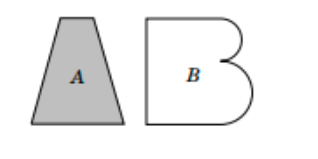
\includegraphics[width=0.6\textwidth]{image//Vocabulaire de theorie des ensembles//1}\end{figure}
The injections $f: A \rightarrow B$ and $g: B \rightarrow A$ are
illustrated in Figure  Think of $f$ as putting a "copy" $f(A)=\{f(x):
x \in A\}$ of $A$ into $B,$ as illustrated. This copy, the range of
$f,$ does not fill up all of $B$ (unless $f$ happens to be
surjective). Likewise, $g$ puts a "copy" $g(B)$ of $B$ into
$A$. Because they are not necessarily bijective, neither $f$ nor $g$
is guaranteed to have an inverse. But the map $g: B \rightarrow g(B)$
from $B$ to $g(B)=\{g(x): x \in B\}$ is bijective, so there is an
inverse $g^{-1}: g(B) \rightarrow B$. (We will need this inverse
soon.)
\begin{figure}[H]\centering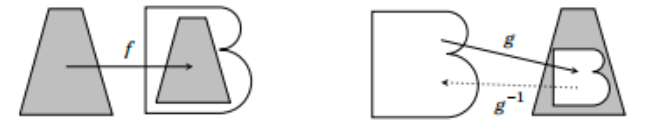
\includegraphics[width=1\textwidth]{image//Vocabulaire de theorie des ensembles//2}\end{figure}
Consider the chain of injections illustrated in the figure below.
\begin{figure}[H]\centering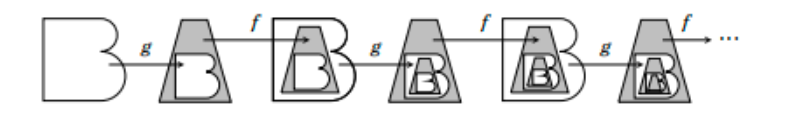
\includegraphics[width=1.2\textwidth]{image//Vocabulaire de theorie des ensembles//3}\end{figure}
 On the left, $g$ puts a copy of $B$ into $A$. Then $f$ puts a copy of $A$ (containing the copy of B) into $B$. Next, $g$ puts a copy of this $B$ -containing- $A$ -containing- $B$ into $A$, and so on, always alternating $g$ and $f$.

The first time $A$ occurs in this sequence, it has a shaded region $A-g(B) .$ In the second occurrence of $A$, the shaded region is $(A-g(B)) \cup(g \circ f)(A-g(B))$. In the third occurrence of $A$, the shaded region is
$$
(A-g(B)) \cup(g \circ f)(A-g(B)) \cup(g \circ f \circ g \circ f)(A-g(B))
$$

To tame the notation, let's say $(g \circ f)^{2}=(g \circ f) \circ(g \circ f)$, and $(g \circ f)^{3}=(g \circ f) \circ(g \circ f) \circ(g \circ f)$, and so on.Let's also agree that $(g \circ f)^{0}=I_{A}$, that is, it is the identity function on $\mathrm{A}$. Then the shaded region of the $n^{th}$ occurrence of $\mathrm{A}$ in the sequence is
$\bigcup\limits_{k=0}^{n-1}(g \circ f)^{k}(A-g(B))$
This process divides A into gray and white regions: the gray region is
$G=\bigcup\limits_{k=0}^{n-1}(g \circ f)^{k}(A-g(B))$
and the white region is $A-G$.
\begin{figure}[H]\centering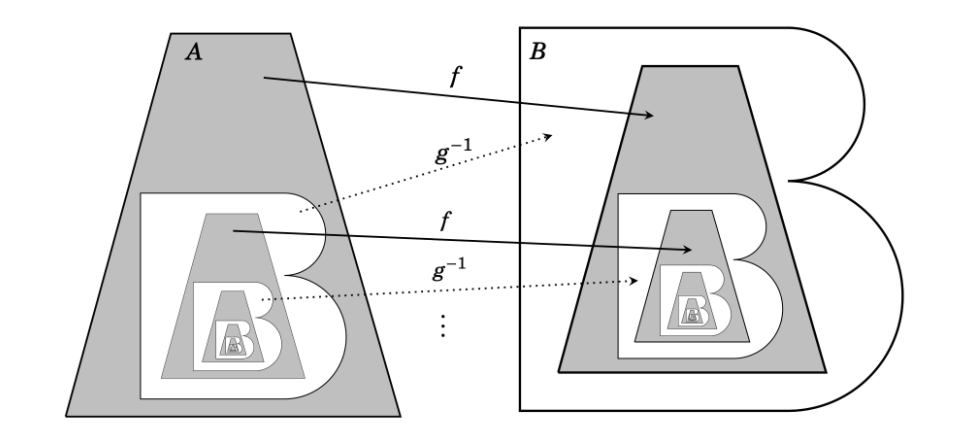
\includegraphics[width=1.2\textwidth]{image//Vocabulaire de theorie des ensembles//4}\end{figure}
The figure suggests our desired bijection $h: A \rightarrow B$. The
injection $f$ sends the gray areas on the left bijectively to the gray
areas on the right. The injection $g^{-1}: g(B) \rightarrow B$ sends
the white areas on the left bijectively to the white areas on the
right. We can thus define $h: A \rightarrow B$ so that $h(x)=f(x)$ if
$x$ is a gray point, and $h(x)=g^{-1}(x)$ if $x$ is a white point.
This informal argument suggests that given injections $f: A \rightarrow B$ and $g: B \rightarrow A$, there is a bijection $h: A \rightarrow B$. But it is not a proof. We now present this as a theorem and tighten up our reasoning in a careful proof, with the above diagrams and ideas as a guide.
\begin{thm}[The Cantor-Bernstein-Schroder Theorem]
If $|A| \leq|B|$ and $|B| \leq|A|,$ then $|A|=|B| .$ In other words, if there are injections $f: A \rightarrow B$ and $g: B \rightarrow A,$ then there is a bijection $h: A \rightarrow B$.
\end{thm}
 \begin{proof}
({\bf Direct})

Suppose there are injections $f: A \rightarrow B$ and $g: B \rightarrow A$. Then, in particular, $g: B \rightarrow g(B)$ is a bijection from B onto the range of $g,$ so it has an inverse $g^{-1}: g(B) \rightarrow B$. (Note that $g: B \rightarrow A$ itself has no inverse $g^{-1}: A \rightarrow B$ unless $g$ is surjective.)

Consider the subset $G=\bigcup\limits_{k=0}^{n-1}(g \circ f)^{k}(A-g(B)) \subseteq A$
Let $W=A-G$, so $A=G \cup W$ is partitioned into two sets G (think gray) and W (think white). Define a function $h: A \rightarrow B$ as
$h(x)=\left\{\begin{array}{cl}f(x) & \text { if } x \in G \\ g^{-1}(x) & \text { if } x \in W\end{array}\right.$
Notice that this makes sense: if $x \in W,$ then $x \notin G,$ so $x \notin A-g(B) \subseteq G,$ hence $x \in g(B),$ so $g^{-1}(x)$ is defined.

To finish the proof, we must show that $\mathrm{h}$ is both injective and surjective.

For injective, we assume $h(x)=h(y),$ and deduce $x=y .$ There are three cases to consider. First, if $x$ and $y$ are both in $G,$ then $h(x)=h(y)$ means $f(x)=f(y),$ so $x=y$ because $f$ is injective. Second, if $x$ and $y$ are both in $W,$ then $h(x)=h(y)$ means $g^{-1}(x)=g^{-1}(y),$ and applying $g$ to both sides gives $x=y$. In the third case, one of $x$ and $y$ is in $G$ and the other is in $W$. Say $x \in G$ and $y \in W$. The definition of G gives $x=(g \circ f)^{k}(z)$ for some $k \geq 0$ and $z$ in $A-g(B)$. Note $h(x)=h(y)$ now implies $f(x)=g^{-1}(y),$ that is, $f\left((g \circ f)^{k}(z)\right)=g^{-1}(y)$. Applying $g$ to both sides gives $(g \circ f)^{k+1}(z)=y,$ which means $y \in G .$ But this is impossible, as $y \in W$. Thus this third case cannot happen. But in the first two cases $h(x)=h(y)$ implies $x=y,$ so $h$ is injective.

To see that $h$ is surjective, take any $b \in B$. We will find an $x \in A$ with $h(x)=b$. Note that $g(b) \in A,$ so either $g(b) \in W$ or $g(b) \in G$. In the first case, $h(g(b))=g^{-1}(g(b))=b,$ so we have an $x=g(b) \in A$ for which $h(x)=b$. In the second case, $g(b) \in G .$ The definition of G shows $g(b)=(g \circ f)^{k}(z)$
for some $z \in A-g(B)$ and $k \geq 0$. In fact we have $k>0,$ because $k=0$ would give $g(b)=(g \circ f)^{0}(z)=z \in A-g(B),$ but clearly $g(b) \notin A-g(B)$. Thus $g(b)=(g \circ f) \circ(g \circ f)^{k-1}(z)=g\left(f\left((g \circ f)^{k-1}(z)\right)\right) .$ Because $g$ is injective, this implies $b=f\left((g \circ f)^{k-1}(z)\right).$Let $x=(g \circ f)^{k-1}(z),$ so $x \in G$ by definition of $G$. Observe that $h(x)=f(x)=f\left((g \circ f)^{k-1}(z)\right)=b$. We have now seen that for any $b \in B$, there is an $x \in A$ for which $h(x)=b$. Thus $h$ is surjective.

Since $h: A \rightarrow B$ is both injective and surjective, it is also bijective.

 \end{proof} 
\begin{proof}
({\bf Indirect})

The existence of $f$ says that ' $A$ is no bigger than $B$ ' and the existence of $g$ says that ' $B$ is no bigger than $A$ '. The conclusion then is that if both hold then ' $A$ and $B$ are the same size'. We shall consider the problem of whether two sets are always comparable in size later.

We consider the mappings $f: P(A) \rightarrow P(B)$ and $g: P(B) \rightarrow P(A)$ determined by $f$ and $g$; they are clearly increasing maps. On the other hand the mapping $C_{A}: P(A) \rightarrow P(A)$ defined by $C_{A}(D)=A \backslash D$ is order reversing, as is the corresponding mapping $C_{B}: P(B) \rightarrow P(B)$. Thus the composite mapping $S=C_{A} \circ g \circ C_{B} \circ f$ is an increasing mapping from $P(A)$ into itself. The Knaster-Tarski fixed-point theorem then tells us that there exists $D \subseteq A$ such that $S(D)=D ;$ the restriction $f_{\mid D}$ of $f$ to $D$ is a bijection of $D$ onto $f(D) .$ Let $E=f(D),$ so that $C_{B}(f(D))=B \backslash E .$ Thus
$$
\begin{aligned}
A \backslash D &=C_{A}(D)=C_{A}(S(D))=C_{A}\left(C_{A} g C_{B} f(D)\right) \\
&\left.=g\left(C_{B} f(D)\right)\right)=g(B \backslash E)
\end{aligned}
$$
Consequently the restriction $g_{\mid B \backslash E}$ of $g$ to $B \backslash E$ is a bijection of $B \backslash E$ onto $A \backslash D ;$ let $k: A \backslash D \rightarrow B \backslash E$ be its inverse. We now set $h(a)=f_{\mid D}(a)$
for $a \in D,$ and set $h(a)=k(a)$ for $a \in A \backslash D ; h$ clearly has the required properties.

\end{proof}

\subsection{Monomorphisms}
There is yet another way to express injectivity, which appears at first more complicated but which is in fact even more basic.

A function $f: A \rightarrow B$ is a monomorphism (or monic) if the following holds:
for all sets $Z$ and all functions $\alpha^{\prime}, \alpha^{\prime \prime}: Z \rightarrow A$
$$
f \circ \alpha^{\prime}=f \circ \alpha^{\prime \prime} \Longrightarrow \alpha^{\prime}=\alpha^{\prime \prime}
$$
\begin{prp}
 A function is injective if and only if it is a monomorphism.
\end{prp}
\begin{proof}
$(\Longrightarrow)$ If a function $f: A \rightarrow B$ is injective, then it has a left-inverse $g: B \rightarrow A$. Now assume that $\alpha^{\prime}, \alpha^{\prime \prime}$ are arbitrary functions from another set $Z$ to $A$ and that
$$
f \circ \alpha^{\prime}=f \circ \alpha^{\prime \prime}
$$
compose on the left by $g,$ and use associativity of composition:
$$
(g \circ f) \circ \alpha^{\prime}=g \circ\left(f \circ \alpha^{\prime}\right)=g \circ\left(f \circ \alpha^{\prime \prime}\right)=(g \circ f) \circ \alpha^{\prime \prime}
$$
since $g$ is a left-inverse of $f,$ this says
$$
\mathrm{id}_{A} \circ \alpha^{\prime}=\mathrm{id}_{A} \circ \alpha^{\prime \prime}
$$
and therefore
$$
\alpha^{\prime}=\alpha^{\prime \prime}
$$
as needed to conclude that $f$ is a monomorphism.

$(\Longleftarrow)$ Now assume that $f$ is a monomorphism. This says something about arbitrary sets $Z$ and arbitrary functions $Z \rightarrow A$; we are going to use a microscopic portion of this information, choosing $Z$ to be any singleton $\{p\}$. Then assigning functions $\alpha^{\prime}, \alpha^{\prime \prime}: Z \rightarrow A$ amounts to choosing to which elements $a^{\prime}=\alpha^{\prime}(p)$, $a^{\prime \prime}=\alpha^{\prime \prime}(p)$ we should send the single element $p$ of $Z$. For this particular choice of $Z$, the property defining monomorphisms, $f \circ \alpha^{\prime}=f \circ \alpha^{\prime \prime} \Longrightarrow \alpha^{\prime}=\alpha^{\prime \prime},$ becomes $$
f \circ \alpha^{\prime}(p)=f \circ \alpha^{\prime \prime}(p) \Longrightarrow \alpha^{\prime}=\alpha^{\prime \prime}
$$
that is,
$$
f\left(a^{\prime}\right)=f\left(a^{\prime \prime}\right) \Longrightarrow \alpha^{\prime}=\alpha^{\prime \prime}
$$
Now two functions from $Z=\{p\}$ to $A$ are equal if and only if they send $p$ to the same element, so this says
$$
f\left(a^{\prime}\right)=f\left(a^{\prime \prime}\right) \Longrightarrow a^{\prime}=a^{\prime \prime}
$$
This has to be true for all $\alpha^{\prime}, \alpha^{\prime \prime},$ that is, for all choices of distinct $a^{\prime}, a^{\prime \prime}$ in $A$. In other words, $f$ has to be injective.

\end{proof} 
\section{Canonical decomposition} 

The reason why we focus our attention on injective and surjective maps is that they provide the basic 'bricks' out of which any function may be constructed.

To see this, we observe that every function $f: A \rightarrow B$ determines an equivalence relation $\sim$ on $A$ as follows: for all $a^{\prime}, a^{\prime \prime} \in A$
$a^{\prime} \sim a^{\prime \prime} \Longleftrightarrow f\left(a^{\prime}\right)=f\left(a^{\prime \prime}\right)$

\begin{thm}\label{t1}
Let $f: A \rightarrow B$ be any function, and define $\sim$ as above. Then $f$ decomposes as follows:
\begin{figure}[H]\centering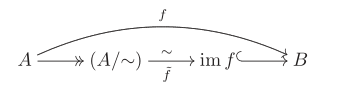
\includegraphics[width=1\textwidth]{image//Vocabulaire de theorie des ensembles//5}\end{figure}
where the first function is the canonical projection $A \rightarrow A / \sim$ (obtained by sending every $a \in A$ to its equivalence class $[a]_{\sim}$), the third function is the inclusion $\operatorname{im} f \subseteq B,$ and the bijection $\tilde{f}$ in the middle is defined by
$$
\tilde{f}\left([a]_{\sim}\right):=f(a)
$$
for all $a \in A.$
\end{thm}
The formula defining $\tilde{f}$ shows immediately that the diagram commutes; so all we have to verify in order to prove this theorem is that

- that formula does define a function:

- that function is in fact a bijection.

The first item is an instance of a class of verifications of the utmost importance. The formula given for $\tilde{f}$ has a colossal built-in ambiguity: the same element in $A / \sim$ may be the equivalence class of many elements of $A$; applying the formula for $\tilde{f}$ requires choosing one of these elements and applying $f$ to it. We have to prove that the result of this operation is independent from this choice: that is, that all possible choices of representatives for that equivalence class lead to the same result. We encode this type of situation by saying that we have to verify that $\tilde{f}$ is well-defined. We will often have to check that the operations we consider are welldefined, in contexts very similar to the one epitomized here.
\begin{proof}

Spelling out the first item discussed above, we have to verify that, for
all $a^{\prime}, a^{\prime \prime}$ in $A$,
$$
\left[a^{\prime}\right]_{\sim}=\left[a^{\prime \prime}\right]_{\sim} \Longrightarrow f\left(a^{\prime}\right)=f\left(a^{\prime \prime}\right) .
$$
Now $\left[a^{\prime}\right]_{\sim}=\left[a^{\prime \prime}\right]_{\sim}$ means that $a^{\prime} \sim a^{\prime \prime},$ and the definition of $\sim$ has been engineered precisely so that this would mean $f\left(a^{\prime}\right)=f\left(a^{\prime \prime}\right)$ as required here. So $\tilde{f}$ is indeed well-defined.

To verify the second item, that is, that $\tilde{f}: A / \sim \rightarrow \operatorname{im} f$ is a bijection, we check explicitly that $\tilde{f}$ is injective and surjective. 

Injective: If $\tilde{f}\left(\left[a^{\prime}\right]_{\sim}\right)=\tilde{f}\left(\left[a^{\prime \prime}\right]_{\sim}\right),$ then $f\left(a^{\prime}\right)=f\left(a^{\prime \prime}\right)$ by definition of $\tilde{f} ;$ hence
$a^{\prime} \sim a^{\prime \prime}$ by definition of $\sim,$ and then $\left[a^{\prime}\right]_{\sim}=\left[a^{\prime \prime}\right]_{\sim} .$ Therefore
$$
\tilde{f}\left(\left[a^{\prime}\right]_{\sim}\right)=\tilde{f}\left(\left[a^{\prime \prime}\right]_{\sim}\right) \Longrightarrow\left[a^{\prime}\right]_{\sim}=\left[a^{\prime \prime}\right]_{\sim}
$$
proving injectivity.

Surjective: Given any $b \in \operatorname{im} f$, there is an element $a \in A$ such that $f(a)=b$. Then
$$
\tilde{f}\left([a]_{\sim}\right)=f(a)=b
$$
by definition of $\tilde{f}$. Since $b$ was arbitrary in $\operatorname{im} f$, this shows that $\tilde{f}$ is surjective, as needed.
\end{proof}
\refthm{t1} shows that every function is the composition of a surjection, followed by an isomorphism, followed by an injection. While its proof is trivial, this is a result of some importance, since it is the prototype of a situation that will occur several times. It will resurface every now and then, with names such as 'the first isomorphism theorem'.
\section{Categories}
The language of categories is affectionately known as abstract nonsense, so named by Norman Steenrod. This term is essentially accurate and not necessarily derogatory: categories refer to nonsense in the sense that they are all about the 'structure', and not about the 'meaning', of what they represent. The emphasis is less on how you run into a specific set you are looking at and more on how that set may sit in relationship with all other sets. Worse (or better) still, the emphasis is less on studying sets, and functions between sets, than on studying 'things, and things that go from things to things' without necessarily being explicit about what these things are: they may be sets, or groups, or rings, or vector spaces, or modules, or other objects that are so exotic that the reader has no right whatsoever to know about them (yet).

'Categories' will intuitively look like sets at first, and in multiple ways. Categories may make you think of sets, in that they are 'collections of objects', and further there will be notions of 'functions from categories to categories' (called functors). At the same time, every category may make you think of the collection of all sets, since there will be analogs of 'functions' among the things it contains.

\begin{dfn}
The definition of a category looks complicated at first, but the gist of it may be summarized quickly: a category consists of a collection of 'objects', and of '{\bf morphisms}' between these objects, satisfying a list of natural conditions.
\end{dfn} 

Note that we refrained from writing a set of objects, opting for the more generic 'collection'. This is an annoying, but unavoidable, difficulty: for example, we want to have a 'category of sets', in which the 'objects' are sets and the 'morphisms' are functions between sets, and the problem is that there simply is not a set of all sets.(That is one thing we learn from Russell’s paradox.) In a sense, the collection of all sets is 'too big' to be a set. There are however ways to deal with such 'collections', and the technical name for them is class. There is a 'class' of all sets (and there will be classes taking care of groups, rings, etc.).

An alternative would be to define a large enough set (called a universe) and then agree that all objects of all categories will be chosen from this gigantic entity. In any case, all we need to know about this is that there is a way to make it work. We will use the term 'class' in the definition, but this will not affect any proof or any other definition. Further, in some of the examples considered below the class in question is a set (we say that the category is small in this case), so we will feel perfectly at home when contemplating these examples.

\begin{dfn}
A category $\mathrm{C}$ consists of

- a class $\operatorname{Obj}(\mathrm{C})$ of objects of the category; and

- for every two objects $A, B$ of $\mathrm{C},$ a set $\operatorname{Hom}_{\mathrm{C}}(A, B)$ of morphisms, with the properties listed below.(注意morphism是我们在之前没有见过的概念,它是由性质定义的抽象对映关系,而且我们在这里还用用集合把它打包了)

As a prototype to keep in mind, think of the objects as 'sets' and of morphisms as 'functions'. This one example should make the defining properties of morphisms look natural and easy to remember:

- For every object $A$ of $\mathrm{C},$ there exists (at least) one morphism $1_{A} \in \operatorname{Hom}_{\mathrm{C}}(A, A)$ the 'identity' on $A$.

- One can compose morphisms: two morphisms $f \in \operatorname{Hom}_{\mathrm{C}}(A, B)$ and $g \in$ $\operatorname{Hom}_{\mathrm{C}}(B, C)$ determine a morphism $g f \in \operatorname{Hom}_{\mathrm{C}}(A, C) .$ That is, for every
triple of objects $A, B, C$ of $\mathrm{C}$ there is a function (of sets)(这里的意思是,因为$\operatorname{Hom}_{\mathrm{C}}(...,...)$是集合,而我们强调在集合上建立的关系叫函数)
$$
\operatorname{Hom}_{\mathrm{C}}(A, B) \times \operatorname{Hom}_{\mathrm{C}}(B, C) \rightarrow \operatorname{Hom}_{\mathrm{C}}(A, C)
$$
and the image of the pair $(f, g)$ is denoted $g f$.

- This 'composition law' is associative: if $f \in \operatorname{Hom}_{\mathrm{C}}(A, B), g \in \operatorname{Hom}_{\mathrm{C}}(B, C)$
and $h \in \operatorname{Hom}_{\mathrm{C}}(C, D),$ then
$$
(h g) f=h(g f)
$$

- The identity morphisms are identities with respect to composition: that is, for all $f \in \operatorname{Hom}_{\mathrm{C}}(A, B)$ we have
$$
f 1_{A}=f, \quad 1_{B} f=f
$$
\end{dfn} 
This is really a mouthful, but again, to remember all this, just think of functions of sets. One further requirement is that the sets
$$
\operatorname{Hom}_{\mathrm{C}}(A, B), \quad \operatorname{Hom}_{\mathrm{C}}(C, D)
$$
be disjoint unless $A=C, B=D ;$ this is something you do not usually think about, but again it holds for ordinary set-functions(We will often use the term ‘set-function’ to emphasize that we are dealing with a function in
the context of sets.). That is, if two functions are one and the same, then necessarily they have the same source and the same target: source and target are part of the datum of a set-function.

A morphism of an object $A$ of a category $\mathrm{C}$ to itself is called an endomorphism; $\operatorname{Hom}_{\mathrm{C}}(A, A)$ is denoted $\operatorname{End}_{\mathrm{C}}(A) .$ One of the axioms of a category tells us that this is a 'pointed' set, as $1_{A} \in \operatorname{End}_{\mathrm{C}}(A)$. We should note that composition defines an 'operation' on $\operatorname{End}_{\mathrm{C}}(A):$ if $f, g$ are elements of $\operatorname{End}_{\mathrm{C}}(A),$ so is their composition $g f$.

Writing '$f \in \operatorname{Hom}_{C}(A, B)$' gets tiresome in the long run. If the category is understood, one may safely drop the index $C,$ or even use arrows as we do with set-functions: $f: A \rightarrow B$. This also allows us to draw diagrams of morphisms in any category; a diagram is said to 'commute' (or to be a 'commutative' diagram) if all ways to traverse it lead to the same results of composing morphisms along the way.

\begin{exm}
Suppose $S$ is a set and $\sim$ is a relation on $S$ satisfying the reflexive and transitive properties. Then we can encode this data into a category:

- objects: the elements of $S$;

- morphisms: if $a, b$ are objects (that is, if $a, b \in S$ ), then let $\operatorname{Hom}(a, b)$ be the set consisting of the element $(a, b) \in S \times S$ if $a \sim b,$ and let $\operatorname{Hom}(a, b)=\emptyset$ otherwise.

Note that (unlike in $\textbf {Set}$($\textbf{Set}$ denote the category of sets.)) there are very few morphisms: at most one for any pair of objects, and no morphisms at all between 'unrelated' objects.

We have to define 'composition of morphisms' and verify that the conditions are satisfied. First of all, do we have 'identities'? If $a$ is an object (that is, if $a \in S)$, we need to find an element
$$
1_{a} \in \operatorname{Hom}(a, a)
$$
This is precisely why we are assuming that $\sim$ is reflexive: this tells us that $\forall a$, $a \sim a ;$ that is, $\operatorname{Hom}(a, a)$ consists of the single element $(a, a) .$ So we have no choice:
we must let
$$
1_{a}=(a, a) \in \operatorname{Hom}(a, a)
$$
As for composition, let $a, b, c$ be objects (that is, elements of $S$ ) and
$$
f \in \operatorname{Hom}(a, b), \quad g \in \operatorname{Hom}(b, c)
$$
we have to define a corresponding morphism $g f \in \operatorname{Hom}(a, c)$. Now,
$$
f \in \operatorname{Hom}(a, b)
$$
tells us that $\operatorname{Hom}(a, b)$ is nonempty, and according to the definition of morphisms in this category that means that $a \sim b,$ and $f$ is in fact the element $(a, b)$ of $S \times S$. Similarly, $g \in \operatorname{Hom}(b, c)$ tells us $b \sim c$ and $g=(b, c) .$ Now
$$
a \sim b \text { and } b \sim c \Longrightarrow a \sim c
$$
since we are assuming that $\sim$ is transitive. This tells us that $\operatorname{Hom}(a, c)$ consists of the single element $(a, c) .$ Thus we again have no choice: we must let
$$
g f:=(a, c) \in \operatorname{Hom}(a, c)
$$
Is this operation associative? If $f \in \operatorname{Hom}(a, b), g \in \operatorname{Hom}(b, c),$ and $h \in \operatorname{Hom}(c, d),$
then necessarily $$
f=(a, b), \quad g=(b, c), \quad h=(c, d)
$$
and
$$
g f=(a, c), \quad h g=(b, d)
$$
and hence
$$
h(g f)=(a, d)=(h g) f,
$$
proving associativity.

The identity morphisms are identities with respect to composition.

The most trivial instance of this construction is the category obtained from a set $S$ taken with the equivalence relation ' $=$; that is, the only morphisms are the identity morphisms. These categories are called {\bf discrete}.
\end{exm}
\begin{exm}
The example is very abstract, but thinking about it will make you rather comfortable with everything we have seen so far; and it is a very common construction.

Let $\mathrm{C}$ be a category, and let $A$ be an object of $\mathrm{C}$. We are going to define a category $\mathrm{C}_{A}$ whose objects are certain morphisms in $\mathrm{C}$ and whose morphisms are certain diagrams of $\mathrm{C}$ (surprise!).

- $\operatorname{Obj}\left(\mathrm{C}_{A}\right)=$ all morphisms from any object of $\mathrm{C}$ to $A$; thus, an object of $\mathrm{C}_{A}$ is a morphism $f \in \operatorname{Hom}_{\mathrm{C}}(Z, A)$ for some object $Z$ of $\mathrm{C}$. Pictorially, an object of $\mathrm{C}_{A}$ is an arrow $Z \stackrel{f}{\rightarrow} A$ in $\mathrm{C} ;$ these are often drawn 'top-down', as in
\begin{figure}[H]\centering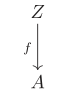
\includegraphics[width=0.1\textwidth]{image//Vocabulaire de theorie des ensembles//6}\end{figure}
What are morphisms in $C_{A}$ going to be? There really is only one sensible way to assign morphisms to a category with objects as above.

- Let $f_{1}, f_{2}$ be objects of $C_{A},$ that is, two arrows in C. 
\begin{figure}[H]\centering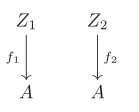
\includegraphics[width=0.2\textwidth]{image//Vocabulaire de theorie des ensembles//7}\end{figure}
Morphisms $f_{1} \rightarrow f_{2}$ are defined to be commutative diagrams in the 'ambient' category $\mathrm{C}$.
\begin{figure}[H]\centering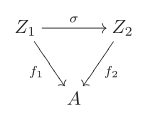
\includegraphics[width=0.3\textwidth]{image//Vocabulaire de theorie des ensembles//8}\end{figure}
That is, morphisms $f_{1} \rightarrow f_{2}$ correspond precisely to those morphisms $\sigma: Z_{1} \rightarrow Z_{2}$ in $C$ such that $f_{1}=f_{2} \sigma$.

The identities are inherited from the identities in $\mathrm{C}$ : for $f: Z \rightarrow A$ in $\mathrm{C}_{A}$, the identity $1_{f}$ corresponds to the diagram which commutes by virtue of the fact that $\mathrm{C}$ is a category(保证了存在性). 
\begin{figure}[H]\centering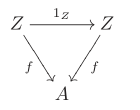
\includegraphics[width=0.3\textwidth]{image//Vocabulaire de theorie des ensembles//9}\end{figure}
Composition is also a subproduct of composition in $\mathrm{C}$. Two morphisms $f_{1} \rightarrow f_{2} \rightarrow f_{3}$ in $\mathrm{C}_{A}$ correspond to putting two commutative diagrams side-by-side:
\begin{figure}[H]\centering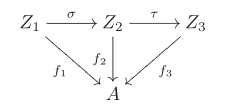
\includegraphics[width=0.4\textwidth]{image//Vocabulaire de theorie des ensembles//10}\end{figure}
And then it follows (again because $\mathrm{C}$ is a category!(保证了复合的可行性)) that the diagram obtained by removing the central arrow also commutes,i.e.,
\begin{figure}[H]\centering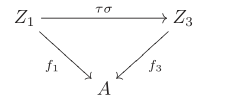
\includegraphics[width=0.4\textwidth]{image//Vocabulaire de theorie des ensembles//11}\end{figure}

Categories constructed in this fashion are called slice categories in the literature; they are particular cases of comma categories.
\end{exm}



































\chapter{Logarithme}
\paragraph{Propriété fondamentale} Une fonction continue strictement monotone sur un intervalle est une bijection de cet intervalle sur son image.


        \paragraph{Exposant rationnel}
        Soit $q\in \mathbb{N*}$.Alors,il est clair que la fonction $\varphi:\mathbb{R_+}\longrightarrow \mathbb{R},\quad x\longmapsto \sqrt[q]{x} $  est continue et strictement croissante.






        \chapter{Vector calculus}
        \section{The vector product(Axial vector)}
        \subsection{Rules of calculation}
        \paragraph{No associativity}
        \textbf{(a$\times$b)$\times$ c $\neq$ a$\times$(b$\times$ c)
        }     The vector on the left side lies in the plane spanned by the vectors \textbf{a} and \textbf{b} (因为the plane spanned by the vectors \textbf{a} and \textbf{b}和 The vector on the left side都与$\mathbf{a}\times\mathbf{b}$垂直) ; the vector on the right side is in the plane spanned by \textbf{b} and \textbf{c}. The subsequent example also shows that associativity does not hold. One has {$\mathbf{e_1}\times( \mathbf{e_2}\times \mathbf{e_2}) =\mathbf{0}$}, but {$(\mathbf{e_1}\times \mathbf{e_2})\times \mathbf{e_2} =\mathbf{-e_1}$}.






\chapter{The natural numbers}
\section{The Peano axioms}

To define the natural numbers,we will use two fundamental concepts: the zero number 0, and the increment operation.



\chapter{Ensembles des nombres réels}
\section{Densité de $\mathbb{Q}$ et de $\mathbb{R\setminus Q}$}
\begin{dfn}
        On dit que'une partie $A\subset \mathbb{R}$ est dense dans $\mathbb{R}$ si :
        $$
        \forall a,b\in \mathbb{R},
        (a<b \Rightarrow A\cap ] a,b [\not=\emptyset )
        $$

\end{dfn}

\begin{prp}{\textbf{caractérisation séquentielle de la densité}}

        Soit A une partie de $\mathbb{R}$, A est dense dans $\mathbb{R}$ ssi pour
        tout $x \in \mathbb{R}$, il existe $(a_n)\in A^{\mathbb{N}}$ une suite d'élément de $A$ qui converge vers x.
\end{prp}

\section{Borne supérieure et borne inférieure}
\begin{dfn}
Soit $(E,\le)$ un ensemble ordonne,A une partie de E.
\begin{itemize}
        \item On dit que A admet une borne supérieure (dans E) si l'ensemble des majorants de A admet un plus petit élément.

        Dans ce cas,ce plus petit élément est appelé la borne supérieure de A et
        est noté $\sup A$
        $$
        \sup A=\min\{M\in E, M \quad majore\quad A\}=\min\{ M\in E  | \forall a\in A ,a\le M\}
        $$

        \item On dit que A admet une borne inférieure (dans E) si l'ensemble des minorants de A admet un plus grand élément.

        Dans ce cas,ce plus grand élément est appelé la borne inférieure de A et
        est noté $\inf A$
                $$
        \inf A=\max\{m\in E, m\text{ minore }A\}=\max\{ m\in E  | \forall a\in A ,m\le a\}
        $$


\end{itemize}
\end{dfn}

\begin{rem}
\textbf{注意sup与max的区别}
\begin{itemize}
\item si A admet un plus grand élément, alors $\max A=\sup A$.
\item Par contre la réciproque est fausse.Par exemple,$[0,1[$ admet une borne supérieure qui est 1 mais pas de plus grand élément
\end{itemize}
\end{rem}



\chapter{Généralités sur les fonctions d'une variable réelle}


\section{Fonctions lipschitziennes}



\begin{dfn}
Soient $f : I \rightarrow \mathbb{K}$ une fonction et $k \in \mathbb{R_{+}^{*}}$. On dit que f est k-lipschitzienne si :
$$\forall x,y \in I ,\left |   f(y)- f(x)\right | \le k \left |   y- x\right |
$$
\begin{itemize}

\item On dit qu'une fonction f est lipschitzienne s'il existe $k > 0$ tel que f soit k-lipschitzienne.
\item Si f est k-lipschitzienne avec $0 < k < 1$, on dit que f est k-{\color{red}contractante}.

\end{itemize}


\end{dfn}

\begin{rem}
La fonction cosinus est 1-lipschitzienne. En effet, soient x et y deux réels, alors :
$$
\begin{aligned}
\left|   \cos(y)-\cos(x)   \right| &=\left|\int_{x}^{y}\cos'(t)\mathrm{d}t \right|\\
&=\left|\int_{x}^{y}-\sin(t)\mathrm{d}t \right|\\
&\le\int_{I}\left|sin(t)\right|\mathrm{d}t&\text{où I = $\left[x, y\right]$ si x $\le$ y et I = $\left[y, x\right]$ sinon}\\
&\le\int_{I}\mathrm{d}t\\
&=\left| y-x \right|\\
\end{aligned}
$$
\end{rem}

\section{Fonctions monotones}

\begin{prp}
Soient $f : I\rightarrow R$ et$ g : J \rightarrow R$ deux applications. On suppose que :
\begin{itemize}
\item f et g sont monotones sur I et J respectivement ;

\item on peut définir la composée $g\circ f$, c'est-à-dire $f(I) \subset J$.
\end{itemize}

Alors la fonction $g\circ f$ est monotone sur I, la monotonie étant donné par \textbf{'la règle des signes'} (croissante : $+$ ,
décroissante : $-$). Autrement dit, si f et g sont de même monotonie, alors $g\circ f$ est croissante et si f et g sont de monotonies opposées, alors  $g\circ f$ est décroissante.
Par ailleurs, si f et g sont strictement monotones, alors  $g\circ f$ l'est aussi.

\end{prp}

\chapter{Étude locale d'une fonction}
\textbf{Cadre} Dans toute la suite, on se restreint à des fonctions définies sur un intervalle réel $I$ ayant au moins deux points, c'est-à-dire tel que $-\infty\le \inf I < \sup I\le \infty$.

On définie alor:
\begin{itemize}
\item L'intérieur de $I$, noté $\mathring{I}=]\inf I,\sup I[$.On a donc dans notre cadre $\mathring{I}\not = \emptyset$
\item L'adhérence de I,notée $\overline{I}$, par $\overline{I}=[\inf I,\sup I]\subset \overline{\mathbb{R}}.$
\end{itemize}
有必要强调,这里用inf和sup来定义区间形态实在比较易混淆,且$I$本身的状态不明确,有时用 $\mathring{I}$和$\overline{I}$只是起到一个确定强调的作用,并不代表$I$需要这么限制或衍生。但是这个I的框架是非常全面的,为了这个全面性,人为地增加了一点抽象度。
\begin{dfn}{\textbf{Voisinage d'un point}}

Soit $a\in \mathbb{R}$.On définit:
\begin{itemize}
        \item  la boule ouverte(respectivement fermée) de centre $a$ et de rayon $\alpha >0$ par $
        B(a,\alpha)=\left\{x\in \mathbb{R},|x-a|< \alpha\right\}$(respectivement $
        B_f(a,\alpha)=\left\{x\in \mathbb{R},|x-a|\le \alpha\right\}$).

        Les ensembles  $
        B(a,\alpha)$ pour $\alpha>0$ sont appelés des voisinages ouverts de $a$ (dans $\mathbb{R}$) et les ensembles $	B_f(a,\alpha)$ sont appelés des voisinages fermés de $a$ (dans $\mathbb{R}$);
        \item un voisinage ouvert (respectivement fermé)
        de $+\infty$ est un intervalle de la forme $]A,+\infty[$(respectivement $[A,+\infty[$) avec $A\in \mathbb{R}$;
                \item un voisinage ouvert (respectivement fermé)
        de $-\infty$ est un intervalle de la forme $]-\infty,A[$(respectivement $]-\infty,A]$) avec $A\in \mathbb{R}$.

\end{itemize}
\textbf{On note $\mathcal{V}_f(a)$ l'ensemble des voisinages fermés de $a$}.
\end{dfn}
值得注意的是,在$a$有限的情况下我们的领域实际上就是boule。另外,$\mathcal{V}_f(a)$是一个邻域的集合,里面的元素不是$x$,而是作为$x$的集合的闭邻域。
\begin{prp}
        $$
        a\in \overline{I}\ \Leftrightarrow \forall V\in \mathcal{V}_f(a),I\cap V\not =\emptyset.
        $$
\end{prp}
\begin{dfn}
Soit $f : I\rightarrow \mathbb{K}$ et $a \in \overline{I}$. On dit qu'une propriété relative à f est vraie au voisinage de a (ou localement en a) s'il existe un voisinage \textbf{ouvert} $\mathcal{B}$ de a telle que la propriété est vraie sur $I \cap \mathcal{B}$.
\end{dfn}

\begin{dfn}{Définition générale de la limite}
        Soient $a\in \overline{I},l\in \overline{\mathbb{R}}$ et $f:I\rightarrow \mathbb{R}.$ On dit que $f$ admet $l$ pour limite en $a$ si:
                $$
                \forall U\in \mathcal{V}_{f}(l),\exists V\in
                \mathcal{V}_{f}(a), \forall x\in I\cap V, f(x)\in U.
                $$
\end{dfn}

\begin{prp}{Limite d'une fonction composée et caractérisation séquentielle de la limite}
Soient $f:I\rightarrow J\subset \mathbb{R}$ et $g:J\rightarrow\mathbb{K}$ deux fonctions, a$\in \overline{I}$.On suppose que :

\begin{itemize}
\item[1.] $\lim_{x\to a}f(x)=l\in \overline{\mathbb{R}};$
\item[2.] $\lim_{x\to l}g(x)=L.$
\end{itemize}

Alors $g\circ f$ admet une limite en $a$ et $\lim_{x\to a}(g\circ f)(x)=L.$

\end{prp}

\chapter{Relation de comparaisons}
\begin{prp}
$f\underset{a}{=}o(g)$ si et seulement si il existe une fonction $h$, définie sur un voisinage $V$ de $a$ telle que $f(x)=g(x)h(x)$ pour tout $x$ dans $V$ et telle que $\lim_{x\to a}h(x)=0$
\end{prp}
\begin{proof}
        \begin{itemize}
\item Montrons $\Rightarrow$

On suppose que $f\underset{a}{=}o(g)$.Prenons pour commencer,$\epsilon=1>0$.Il existe alors un voisinage ouvert $V_1$ de $a$ tel que: ($\star$) $\forall x\in I\cap V_1,\left |f(x)\right |\le \left |g(x)\right |$ .

On définit alors la fonction $h$ sur $I\cap V_1$ par:
\begin{equation*}
h(x)=
\begin{cases}
\frac{f(x)}{g(x)} &\mbox{si $g(x)\not=0$}\\
0 &\mbox{si $g(x)=0$}\\
\end{cases}
\end{equation*}
        \end{itemize}
\end{proof}



        \chapter{Suites réelles et complexes}
        \section{Suite de nombres réels}
        \subsection{Définition}
        On appelle suite de nombre réels une fonction $u:\mathbb{N}\to\mathbb{R}$. Pour tout entier n, on note $u(n) = u_n$.
        On note alors $u = (u_n)_{n\in\mathbb{N}}$ la suite u et $\mathbb{R}^\mathbb{N}$ l'ensemble des suites réelles.


        Si u est une suite, on appelle $u_n$ le nième \textcolor{red}{terme} de la suite u (ou terme d'indice ou de rang n). La suite u est alors notée $(u_n)_{n\in N}$ ou $(u_n)$ plus simplement.Par extension, nous appellerons aussi suite réelle une famille de réels indexée par un intervalle d'entiers
        du type $\llbracket n_0, + \infty \llbracket$ .La suite u est dans ce cas notée $(u_n)_{n\ge n_0}$ .

        Une suite peut être  définie de trois manières différentes :
        \\1.par une formule explicite : chaque terme de la suite est donné directement en fonction de n, soit $u_n = f(n)$.
        \\2.par une formule de récurrence : $u_n$ est exprimé en fonction de n et des termes précédents : $u_{n−1}, ... ,u_0$
        \\3.par une formule implicite : le terme général un de la suite est solution d’une équation dépendant de n. Par exemple,

        $\forall n \in \mathbb{N}$, $u_n$ est l'unique solution de l'équation $x^3+x-1=n$


        \paragraph{rang et suite stationnaire}
        On dit qu'une suite $(u_n)$ satisfait la propriété $P(n)$ à partir d'un certain rang s'il existe $n_0 \in \mathbb{N}$ tel que
        $\forall n \ge n_0, P(n)$ est vraie.

        La suite $(u_n)$ est dite stationnaire si elle est constante à partir d’un certain rang i.e si :
        $\exists n_0 \in \mathbb{N}, \forall n \ge n_0, u_n = u_{n_0}$ .

        Exemple: La suite $(u_n)$ définie par $u_n = \prod _{k=0}^n(100-k)$ est stationnaire, constante égale à 0 à partir du rang n = 100.

\paragraph{Théorème(basic) de la relation équivalante}
Soient $(u_n)_{n\in \mathbb{N}}$ et  $(v_n)_{n\in \mathbb{N}}$  deux suite complexes ne s'annulant pas à partir d'un certain rang.
$$u_n\underset{+\infty}{\sim} v_n \Longleftrightarrow  u_n \underset{+\infty}{=} v_n + o(v_n).$$
\begin{proof}
        $$u_n\underset{+\infty}{\sim} v_n \Longleftrightarrow  \frac{u_n}{v_n}\xrightarrow[+\infty]{} 1 \Longleftrightarrow  \frac{u_n}{v_n}
\underset{+\infty}{=} 1+o(1)
\Longleftrightarrow  u_n
\underset{+\infty}{=} v_n+v_no(1)
\Longleftrightarrow u_n \underset{+\infty}{=} v_n + o(v_n).$$
(car $\frac{v_no(1)}{v_n}=o(1)\xrightarrow[+\infty]{} 0$)


\end{proof}

        %2020/7/14 终 待改进及补充
        %2020/7/25 第一次补充



        %这是一个插入节,中间跳了不少内容,纯粹是因为觉得好玩拿出来提前码

        %2020/7/15起

        \subsection{Séries}
Définition: Soit u dans	$\mathbb{R}^\mathbb{N}$
On appelle série de terme général $ (u_n)_{n\in\mathbb{N}}$ \textcolor{red}{la suite} S $\in$ $\mathbb{R}^\mathbb{N}$ définie par :
\begin{equation*}
\forall n \in \mathbb{R} , S_n = \sum_{k=0}^{n}u_k.
\end{equation*}
On note aussi $\sum u_k$ \textcolor{red}{la suite} S de terme général $ (u_n)_{n\in\mathbb{N}}$.


这里非常秀的是将级数定义的像是一个与另一个数列挂钩的数列,完全刷新了我以前对级数的认识。从而将级数划归到了实数列的
研究范围。所以我们可以借助数列发散收敛的相关成果来研究一下级数的发散收敛问题。但是这里有一个非常技巧性的,用于确定级数范围(是否有界)的方法(Comparaison avec une intégrale,其实就是一个不等式),同时它也可以给出一个关于级数的行为的很好的“点子”,即给出它的等价(对发散级数)。Ce genre de méthode va marcher quand on étudie une série de terme général $(f(k))_{k\in \mathbb{N}}$ avec f une fonction \textcolor{red}{monotone et continue}.


下面举一个判定级数收敛性的例子,方法是用`单调有界数列收敛’这一性质去判断。即先研究单调性,再研究有界性。


Exemple:Montrer que la série de terme général $(\frac{1}{(n+1)^2})_{n \in \mathbb{N}}$ converge.
\begin{proof}
        Ici, $\forall$ n $\in$ $\mathbb{N}$, $S_n$ = $\sum_{k=0}^{n} {\frac{1}{(k+1)^2}}$.
        \\Pour tout n dans $\mathbb{N}$,
        \begin{equation*}
        S_{n+1}-S_n=\sum_{k=0}^{n+1} {\frac{1}{(k+1)^2}}-\sum_{k=0}^{n} {\frac{1}{(k+1)^2}}=\frac{1}{(n+2)^2}\ge{0}.
        \end{equation*}
        La suite S est donc croissante.\\
        De plus, pour k dans $\mathbb{N^*}$, la fonction $ t\longmapsto \frac{1}{t^2} $ est décroissante sur [k,k+1],donc:
        \begin{equation*}
        \forall t \in [k,k+1], \frac{1}{(k+1)^2} \leqslant \frac{1}{t^2}
        \end{equation*}
        Pour k dans $\mathbb{N^*}$,
        la fonction  $ t\longmapsto \frac{1}{t^2} $ est continue sur [k,k+1].Intégrant l’inégalité précédentes, on obtient :
        \begin{equation*}
        \forall t \in [k,k+1],
        \frac{1}{(k+1)^2} = \int_k^{k+1} \frac{1}{(k+1)^2}\,\mathrm{d}t
        \leqslant \int_k^{k+1} \frac{1}{t^2}\,\mathrm{d}t=
        \frac{1}{k}-\frac{1}{k+1}
        \end{equation*}
        这一步利用了积分的保号性,不等式两边同时乘上$\mathrm{d}t$后对t求和(即对t积分)这里注意$\frac{1}{(k+1)^2}$与积分变量t无关,而积分的上下限选取又恰好是一个长度为1的区间从而我们保证了左边我们研究的项在积分后不变而右边变成了积分的形式,从而得到了一个新的限制关系(同一个量同时满足小于一个函数和它的积分)。\textcolor{red}{事实上,我们只是利用这种操作来得到一个放缩的灵感,来从无到有的人为构建放缩不等式,这时我们利用右边构建的定积分写成了一个可以求和的”差项“级数,即前后项可以互相抵消一部分。}


        On obtient donc que pour tout n dans $\mathbb{N^*}$,
        \begin{equation*}
        S_n=1+\sum_{k=1}^{n} {\frac{1}{(k+1)^2}}
        \leqslant 1+(1-\frac{1}{n+1})
        \leqslant 2
        \end{equation*}
        La suite S est croissante et majorée, donc converge.\\
        Conclusion : la série de terme général $(\frac{1}{(n+1)^2})_{n \in \mathbb{N}}$ converge.
\end{proof}

Remarque:“积分比较”不但可以确定一个级数收敛,也可以给出级数和的一组上下界,
$$
\forall t \in [k,k+1], \frac{1}{t^2} \leqslant \frac{1}{k^2}
$$
On obtient :
\begin{equation*}
\forall t \in [k,k+1],
\frac{1}{k^2} = \int_k^{k+1} \frac{1}{t^2}\,\mathrm{d}t=
\frac{1}{k}-\frac{1}{k+1}
\leqslant \frac{1}{k^2} = \int_k^{k+1} \frac{1}{k^2}\,\mathrm{d}t
\end{equation*}
Soit:
$$\frac{1}{n^{2}}+(1-\frac{1}{n+1})
\leqslant S_n=\frac{1}{n^{2}}+\sum_{k=1}^{n} {\frac{1}{k^2}}
$$
取极限后,我们最终得到级数和的范围在1和2之间.

\paragraph{Théorème de Césaro}
这个定理给出了一种特殊级数和其项数列的收敛关系。我们先给出这种特殊的级数:

Définition:  Soit $(u_n)_{n\in \mathbb{N}}$ une suite réelle;on lui associe la suite $(v_n)_{n\in \mathbb{N}}$ définie par :
$$ v_0=u_0 \quad et \quad \forall n \in \mathbb{N*}, v_n=\frac{u_1+u_2+...+u_n}{n} $$
La suite $(v_n)_{n\in \mathbb{N}}$ est appelée moyenne de Césaro de la suite $(u_n)_{n\in \mathbb{N}}$.

Théorème: Si la suite $(u_n)_{n\in \mathbb{N}}$ converge vers l alors La suite $(v_n)_{n\in \mathbb{N}}$ converge aussi vers l

\begin{proof}
        Soit $\epsilon > 0$ fixé, on veut montrer que $ \exists N=N(\epsilon) \in \mathbb{N} $ tel que $n\ge N$ on ait $|v_n-l| < \epsilon$.

        Or par hypothèse $\lim_{n \rightarrow \infty} u_n = l $,donc:

        $ \exists p=p(\epsilon) \in \mathbb{N} $ tel que $n\ge p$ on ait $|u_n-l| < \frac{\epsilon}{2}$

        On a pour tout $n\ge p$,
        \begin{align}
        v_n-l ={} & \frac{u_1+u_2+...+u_n}{n}-l \notag \\
        ={} & \frac{u_1+u_2+...+u_p+u_{p+1}+...+u_n-nl}{n} \notag \\
        ={} & \frac{(u_1-l)+(u_2-l)+...+(u_p-l)+(u_{p+1}-l)+...+(u_n-l)}{n}  \notag \\
        ={} & \frac{(u_1-l)+(u_2-l)+...+(u_p-l)}{n}+\frac{(u_{p+1}-l)+...+(u_n-l)}{n}  \notag
        \end{align}
        En vertu de l'inégalité triangulaire :
        $$|v_n-l| \le \frac{1}{n}\sum_{k=1}^{p}|u_k-l| + \frac{1}{n}\sum_{k=p+1}^{n}|u_k-l|.
        $$
        En posant
        $$C=\frac{1}{n}\sum_{k=1}^{p}|u_k-l|$$
        (notons que C est une constante indépendante de n) et puisque $|u_k-l|< \frac{\epsilon}{2}$
        pour tout k $\ge$ p, on a :
        \begin{align}
        |v_n-l| \le & \frac{C}{n} + \frac{n-p}{n}\frac{\epsilon}{2}. \notag \\
              \le & \frac{C}{n} + \frac{\epsilon}{2}\quad(car\quad \frac{n-p}{n} < 1). \notag
        \end{align}
        Par ailleurs, $\lim_{n\rightarrow \infty}\frac{C}{n}=0$ donc

$ \exists q=q(\epsilon) \in \mathbb{N} $ tel que $n\ge q$ on ait $|\frac{C}{n}|=\frac{C}{n} < \frac{\epsilon}{2}$

Donc,en prenant $N=max(p,q)$, on a finalement:

$ \exists N=N(\epsilon) \in \mathbb{N} $ tel que $n\ge N$ on ait $|v_n-l| < \epsilon$.

\end{proof}
%2020/7/15终,待改进及补充

%依然是一个有意思的数学证明,与上面的之间跳过了很多内容,待补充
\paragraph{Théorème de Bolzano-Weierstrass}
Soit u dans $\mathbb{R}^\mathbb{N}$ une suite bornée. Alors, il existe une suite extraite de u qui est convergente.
\begin{proof}
Soit u une suite bornée. Pour commencer, je définie un ensemble $\mathfrak{BW}$:
\begin{equation*}
\mathfrak{BW} = \{n_0 \in \mathbb{N}|\forall n \ge n_0 \Longrightarrow u_{n} \leqslant u_{n_0} \}
\end{equation*}
这里定义出$\mathfrak{BW}$(BW代表Bolzano-Weierstrass)是第一次extraction的像集,这个extraction做了这样一次抽取即,使得它的像集的元素及其对应的u中的项暗含了一个递减数列。从这个比较抽象和模糊的集合出发我们根据它是无限集和有限集分两种情况,用数学归纳法来分别定义两个对映的具体的extraction(能用数学归纳法来定义的也只有以$\mathbb{N}$为出发集的函数了)。
\subparagraph{Cas1}
l’ensemble $\mathfrak{BW}$ est infini.

Je définis une fonction $\mathbb{N}\xrightarrow{\varphi} \mathbb{N}$ par récurrence en posant :
\begin{equation*}
\varphi(0)=inf\{n \in \mathfrak{BW}\}
\end{equation*}
$\mathfrak{BW}$ est un ensemble d’entiers non-vide, donc il contient un plus petit élément qui est dans $\mathbb{N}$ et
$\varphi(0) \in \mathbb{N}$.


$\varphi(k)$ étant défini, on pose :
\begin{equation*}
\varphi(k+1)=inf\{n \in \mathfrak{BW}\backslash \{\varphi(0),...,\varphi(k)\}\}
\end{equation*}
On construit ainsi par récurrence une extraction $\varphi$.
 $\mathfrak{BW}\backslash \{\varphi(0),...,\varphi(k)\}$ d’entiers non-vide (car sinon $\mathfrak{BW}$ est fini), donc il contient un plus petit élément qui est dans $\mathbb{N}$ et $\varphi(k+1) \in \mathbb{N}$ et $\varphi(k+1) \ge \varphi(k)$.

 上面的最后一条关系是利用了以下原理:$\varphi(k) , \varphi(k+1) \in \mathfrak{BW}\backslash \{\varphi(0),...,\varphi(k-1)\}$,
 但是$\varphi(k)$却做了这个集合的下界,从而一定有$\varphi(k+1) \ge \varphi(k)$。

La suite $(u_{\varphi(n)})_{n\in \mathbb{N}}$ est minorée puisque u est minorée. La suite est également décroissante. 因为$(\varphi(n))_{n\in \mathbb{N}}$
在集合$\mathfrak{BW}$里,而集合$\mathfrak{BW}$的定义是一个性质定义,它的每一个元素对映的u中的项是所有比它大的元素对映的u中的项中最大的。所以,元素越小的对应的u中的项就越大。
这里的这个结论也可以直接由定义中的逻辑命题和单调递减数列判定命题结合得出。
La suite $(u_{\varphi(n)})_{n\in \mathbb{N}}$ est donc décroissante et minorée, donc converge.
\subparagraph{Cas2}
l’ensemble $\mathfrak{BW}$ est fini ,je note N son plus grand élément (si par hasard M est vide,这时N取谁是任意选取的, je prends N = 0,).因为收敛是无穷数列的性质,所以这里$\mathfrak{BW}$已经不再是我们需要的extraction了,同样这也绝了我们想要构建一个递减无穷数列的念头。但这里我们没有必要再建立一个抽象的extraction而是利用这种对递减数列的排除直接在$\mathfrak{BW}$外(这个外只能指majorant,因为无穷数列的指标都要递增往正无穷)用数学归纳法搭建一个逐项递增的无穷数列。 On définit une extraction
$\mathbb{N}\xrightarrow{\varphi} \mathbb{N}$ par récurrence en posant $\varphi(0)=N+1$. $N + 1 \notin \mathfrak{BW}$.
$\varphi(k)$ étant construit, on pose :
\begin{equation*}
\varphi(k+1)=inf\{n \in \llbracket \varphi(k)+1 , + \infty \llbracket
 ,u_{\varphi(k+1)} \ge u_{\varphi(k)} \}
\end{equation*}
这个集合永远非空,因为我们所选的元素都不在
$\mathfrak{BW}$中,等于说是对$\mathfrak{BW}$中性质命题的否定,然后我们会得到一个关于存在性(任意的否定)的结论。
另外在用数学归纳法构建extraction时,inf是一个很好用的逐项筛选工具,只要在其后把我们需要的集合范围加上,我们就等于确定了一个抽象且合理的对象(项)。La suite  $(u_{\varphi(n)})_{n\in \mathbb{N}}$  est croissante. La suite $(u_{\varphi(n)})_{n\in \mathbb{N}}$ est aussi majorée, donc cette suite converge.

Dans tous les cas, on a donc construit une suite extraite convergente, ce qui prouve le théorème de Bolzano-Weierstrass.
\end{proof}

\chapter{Infinite series}
The notion of convergence of a sequence allows us to consider infinite sums, or series. Once again, we take either $\mathbf{N}$ or $\mathbf{Z}^{+}$ as index set. We shall generally consider the case where the terms of the series are complex-valued; since $\mathbf{R} \subseteq$ C, the results will also apply to the case where all the terms are real-valued. Suppose that $\left(z_{j}\right)_{j=0}^{\infty}$ is a sequence of complex numbers. We set
$$
s_{n}=\sum_{j=0}^{n} z_{j}=z_{0}+\cdots+z_{n}
$$
where $s_{n}$ is the $n$ th partial sum. If $s_{n} \rightarrow s$ as $n \rightarrow \infty$, we say that the infinite sum, or infinite series, $\sum_{j=0}^{\infty} z_{j}$ converges to $s .$ If $s_{n}$ does not converge, then we say that $\sum_{j=0}^{\infty} z_{j}$ diverges.

Here are two easy examples: as we shall see, the first one is particularly useful. Suppose that $|z|<1 .$ Let $z_{j}=z^{j}$ for $j \in \mathbf{Z}^{+} .$ Then
$$
(1-z) s_{n}=\left(1+z+\cdots+z^{n}\right)-\left(z+z^{2}+\cdots+z^{n+1}\right)=1-z^{n+1}
$$
so that
$$
s_{n}=\frac{1-z^{n+1}}{1-z}=\frac{1}{1-z}-\frac{z^{n+1}}{1-z} \text { and } s_{n} \rightarrow \frac{1}{1-z} \text { as } n \rightarrow \infty
$$
Thus $\sum_{j=0}^{\infty} z^{j}=1 /(1-z).$

Secondly, let
$$
a_{j}=\frac{1}{j(j+1)}=\frac{1}{j}-\frac{1}{j+1} \text { for } j \in \mathbf{N}
$$
Then
$$
s_{n}=\sum_{j=1}^{n} a_{j}=\left(1-\frac{1}{2}\right)+\left(\frac{1}{2}-\frac{1}{3}\right)+\cdots+\left(\frac{1}{n}-\frac{1}{n+1}\right)=1-\frac{1}{n+1}
$$
so that $s_{n} \rightarrow 1: \sum_{j=1}^{\infty} 1 / j(j+1)=1$.
We can apply the results that we have obtained about convergent sequences to infinite series. For example, a complex series is convergent if and only if the sum of the real parts and the sum of the imaginary parts of the terms both converge.
\begin{prp}
Suppose that $z_{j}=x_{j}+i y_{j}$ and that $s=\sigma+i \tau .$ Then $\sum_{j=0}^{\infty} z_{j}$ converges to $s$ if and only if $\sum_{j=0}^{\infty} x_{j}$ converges to $\sigma$ and $\sum_{j=0}^{\infty} y_{j}$ converges to $\tau$.
\end{prp}
\begin{thm}
	Suppose that $\sum_{j=0}^{\infty} z_{j}$ converges to $s$ and that $\sum_{j=0}^{\infty} w_{j}$ converges to $t .$
	
	(i) When it exists, the sum is unique: if $\sum_{j=0}^{\infty} z_{j}=s^{\prime},$ then $s=s^{\prime}$.
	
	(ii)$\sum_{j=0}^{\infty}\left(z_{j}+w_{j}\right)$ converges to $s+t$.
	
	(iii) If $c \in \mathbf{C}$ then $\sum_{j=0}^{\infty} c z_{j}$ converges to cs.
	
	(iv) If $z_{j}$ and $w_{j}$ are real, and $z_{j} \leq w_{j}$ for all $j,$ then $s \leq t$.
\end{thm}

Suppose that $\left(j_{k}\right)_{k=0}^{\infty}$ is a strictly increasing sequence in $\mathbf{Z}^{+} .$ Set $b_{0}=$ $\sum_{j=0}^{j_{0}} z_{j},$ and set $b_{k}=\sum_{j=j_{k-1}+1}^{j_{k}} z_{j}$ for $k>0 .$ Then the sequence $\left(b_{k}\right)_{k=0}^{\infty}$
is called a block sequence, or bracketed sequence, derived from $\left(a_{j}\right)_{j=0}^{\infty} .$ 
\begin{prp}
If $\sum_{j=0}^{\infty} z_{j}$ converges to $s$ and $\left(b_{k}\right)_{k=0}^{\infty}$ is a block sequence derived from it, then $\sum_{k=0}^{\infty} b_{k}$ converges to $s$.
\end{prp} 
The converse is false in general. Let $z_{j}=$ $(-1)^{j},$ for $j \in \mathbf{N}^{+} .$ Then $s_{2 n}=0$ and $s_{2 n+1}=1$ for all $n \in \mathbf{Z}^{+},$ so that $\sum_{j=0}^{\infty} z_{j}$ diverges. If we set $j_{k}=2 k+1,$ then $b_{k}=z_{2 k}+z_{2 k+1}=0$ for $k \in \mathbf{N}^{+},$ so that $\sum_{k=1}^{\infty} b_{k}$ converges to 0 We also have the following simple result.
\begin{prp}
If $\sum_{j=0}^{\infty} z_{j}$ converges, then $z_{j} \rightarrow 0$ as $j \rightarrow \infty$
\end{prp}
 \begin{proof}
 Suppose that the sum is $s$. Then $s_{j} \rightarrow s$ and $s_{j-1} \rightarrow s$ as $j \rightarrow \infty,$ so that $z_{j}=s_{j}-s_{j-1} \rightarrow 0$ as $j \rightarrow \infty$.
 \end{proof}

The general principle of convergence takes the following form.
\begin{thm}[The general principle of convergence]Suppose that  $\left(z_{j}\right)_{j=0}^{\infty}$ is a sequence of complex numbers. Then $\sum_{j=0}^{\infty} z_{j}$ converges if and only if given $\epsilon>0$ there exists $n_{0}$ such that $\left|s_{n}-s_{m}\right|=\left|\sum_{j=m+1}^{n} z_{j}\right|<\epsilon$ for $n>m \geq n_{0}$.
\end{thm}
\section{Series with non-negative terms}
Series with real non-negative terms behave particularly well.
\begin{thm}
Suppose that $\left(a_{j}\right)_{j=0}^{\infty}$ is a sequence of non-negative real numbers, and that $s_{n}=\sum_{j=1}^{n} a_{j} .$ Then $\left(s_{n}\right)_{n=0}^{\infty}$ is an increasing sequence.

 Either $\left(s_{n}\right)_{n=0}^{\infty}$ is bounded, in which case $\sum_{j=0}^{\infty} a_{j}$ converges to $\sup _{n} s_{n},$ or $s_{n} \rightarrow \infty,$ in which case we say that $\sum_{j=0}^{\infty} a_{j}$ diverges to $+\infty,$ and write $\sum_{j=0}^{\infty} a_{j}=+\infty$
\end{thm} 

This theorem indicates that summing a series of non-negative terms is reasonably straightforward. Here are some of its consequences; the first is one of many tests for convergence.

\begin{cor}[The comparison test]
$\quad$ If $0 \leq c_{j} \leq a_{j}$ for all $j \geq j_{0}$ and $\sum_{j=0}^{\infty} a_{j}$ converges then $\sum_{j=0}^{\infty} c_{j}$ converges, and $\sum_{j=0}^{\infty} c_{j} \leq \sum_{j=0}^{\infty} a_{j}.$
\end{cor} 
For example, $\sum_{j=1}^{\infty} 1 / j^{2}$ converges, since $1 / j^{2} \leq 2 / j(j+1)$. Note that this corollary does not tell us what the sum is, although we can deduce that it is at most $2 .$ (In fact the sum is $\pi^{2} / 6$; we shall prove this much later!)
\begin{cor}
If $\left(a_{j}\right)_{j=0}^{\infty}$ is a sequence of non-negative numbers and $\left(b_{k}\right)_{k=0}^{\infty}$ is a block sequence derived from it, then $\sum_{j=1}^{\infty} a_{j}$ converges to $s$ if and only if $\sum_{k=1}^{\infty} b_{k}$ converges to $s$.
\end{cor}
\begin{proof}
$s_{n} \rightarrow s$ as $n \rightarrow \infty$ if and only if $s_{j_{l}} \rightarrow s$ as $l \rightarrow \infty,$ and $s_{j_{l}}=$ $\sum_{k=0}^{l} b_{k}$
\end{proof}
We can say more when $\left(a_{j}\right)_{j=0}^{\infty}$ is a decreasing sequence of non-negative numbers.
\begin{cor}[The compression principle]
If $\left(a_{j}\right)_{j=1}^{\infty}$ is a decreasing sequence of non-negative real numbers, then $\sum_{j=1}^{\infty} a_{j}$ converges if and only if $\sum_{k=0}^{\infty} 2^{k} a_{2^{k}}$ converges. If so then
$$
\frac{1}{2} \sum_{k=0}^{\infty} 2^{k} a_{2^{k}} \leq \sum_{j=0}^{\infty} a_{j} \leq \sum_{k=0}^{\infty} 2^{k} a_{2^{k}}
$$
\end{cor}
\begin{proof}
Let $\left(b_{k}\right)_{k=0}^{\infty}$ be the block sequence obtained by taking $j_{k}=2^{k} .$ Then
$$
\frac{1}{2} 2^{k} a_{2^{k}}=2^{k-1} a_{2^{k}} \leq b_{k}=a_{2^{k-1}+1}+\cdots+a_{2^{k}} \leq 2^{k-1} a_{2^{k-1}}
$$
since $\left(a_{j}\right)_{j=0}^{\infty}$ is decreasing, and there are $2^{k-1}$ summands.
\end{proof}
\begin{cor}[The harmonic series]
$\sum_{j=1}^{\infty} 1 / j$ diverges to $+\infty$.
\end{cor}  
\begin{proof}
For if $a_{j}=1 / j$ then $2^{k} a_{2^{k}}=1,$ so that the result follows from the preceding corollary.
\end{proof}

 \begin{cor}[Cauchy's test]
 Suppose that $\left(a_{j}\right)_{j=0}^{\infty}$ is a bounded sequence of non-negative real numbers. If $\lim \sup _{j \rightarrow \infty} a_{j}^{1 / j}<1$ then $\sum_{j=1}^{\infty} a_{j}$
converges, and if $\limsup _{j \rightarrow \infty} a_{j}^{1 / j}>1$ then $\sum_{j=1}^{\infty} a_{j}=+\infty .$
 \end{cor}
\begin{proof}
In the first case, choose $r$ such that $\limsup _{j \rightarrow \infty} a_{j}^{1 / j}<r<1 .$ Then there exists $j_{0}$ such that $a_{j}^{1 / j}<r$ for $j \geq j_{0}$. Thus $a_{j} \leq r^{j}$ for $j \geq j_{0}$ and so, using the comparison test, $\sum_{j=1}^{\infty} a_{j}$ converges.

In the second case, for each $j \in \mathbf{Z}^{+}$ there exists $k \geq j$ such that $a_{k}^{1 / k}>1$ so that $a_{k}>1$. Thus $\left(a_{j}\right)_{j=0}^{\infty}$ is not a null sequence and so $\sum_{j=1}^{\infty} a_{j}$ diverges to $+\infty$.
\end{proof}
\begin{cor}[D'Alembert's ratio test]
Suppose that $\left(a_{j}\right)_{j=0}^{\infty}$is a sequence of positive real numbers. If $\lim \sup _{j \rightarrow \infty} a_{j+1} / a_{j}<1$ then $\sum_{j=1}^{\infty} a_{j}$
converges. If $\lim \inf _{j \rightarrow \infty} a_{j+1} / a_{j}>1$ then $\sum_{j=1}^{\infty} a_{j}$ diverges to $+\infty$
\end{cor}
\begin{proof}
	In the first case, choose $r$ such that $\lim \sup _{j \rightarrow \infty} a_{j+1} / a_{j}<r<1$. Then there exists $j_{0}$ such that $a_{j+1} / a_{j}<r$ for $j \geq j_{0} .$ Thus if $j>j_{0}$ then
	$$
	a_{j}=\left(\frac{a_{j}}{a_{j-1}}\right)\left(\frac{a_{j-1}}{a_{j-2}}\right) \ldots\left(\frac{a_{j_{0}+1}}{a_{j_{0}}}\right) a_{j_{0}} \leq r^{j-j_{0}} a_{j_{0}}=\left(a_{j_{0}} r^{j_{0}}\right) r^{j}
	$$
	and so, taking the terms $a_{1}, \ldots, a_{j_{0}}$ into account, there exists $M$ such that $a_{j} \leq M r^{j}$ for all $j .$ By the comparison test, $\sum_{j=1}^{\infty} a_{j}$ converges.
	
	In the second case, there exists $j_{1}$ such that $a_{j+1}>a_{j}$ for $j \geq j_{1},$ so that $a_{j} \geq a_{j_{1}}$ for $j \geq j_{1}$. Thus $\left(a_{j}\right)_{j=0}^{\infty}$ is not a null sequence, so that $\sum_{j=1}^{\infty} a_{j}$ diverges to $+\infty$.
\end{proof}
It is important to note that neither corollary gives any information when $\limsup _{j \rightarrow \infty} a_{j}^{1 / j}=1$ or when $\limsup _{j \rightarrow \infty} a_{j} / a_{j+1}=1 .$ When $a_{j}=1 / j$
the sum diverges, and when $a_{j}=1 / j^{2},$ the sum converges. In either case,
$$
a_{j}^{1 / j} \rightarrow 1 \text { and } a_{j+1} / a_{j} \rightarrow 1 \text { as } j \rightarrow \infty
$$
We use D'Alembert's ratio test to introduce the exponential function, one of the most important functions in analysis. Suppose that $x \geq 0 .$ Let $a_{j}=x^{j} / j !$. Then $a_{j+1} / a_{j}=x /(j+1)$ and $x /(j+1) \rightarrow 0$ as $j \rightarrow \infty$
so that $\sum_{j=0}^{\infty} x^{j} / j !$ converges, to $\exp (x),$ say. The mapping $x \rightarrow \exp (x)$ is the exponential function. We set $e=\exp (1)=\sum_{j=0}^{\infty} 1 / j ! .$ Note that since $1 / n ! \leq 1 / 2^{n-1},$ it follows that
$$
2 \leq e \leq 1+\sum_{j=1}^{\infty} \frac{1}{2^{j-1}}=3
$$
In fact, $e=2.718281828 \ldots .$ We shall extend this definition for negative $x$ and for complex $x$.

 Suppose that $x$ is a positive real number.We set $x_{n}=\left\lfloor 2^{n} x\right\rfloor / 2^{n}$. Let $a_{0}=x_{0}=\lfloor x\rfloor$ and let $a_{n}=2^{n}\left(x_{n}-x_{n-1}\right)$ for $n \in \mathbf{N} .$ Then $a_{n}=0$ or 1 and
$$
x_{n}=a_{0}+\left(\frac{a_{1}}{2}+\frac{a_{2}}{2^{2}}+\cdots+\frac{a_{n}}{2^{n}}\right)
$$
Thus $x=\sum_{n=0}^{\infty}\left(a_{n} / 2^{n}\right) .$ We can write this as
$x=a_{0} \cdot a_{1} a_{2} \ldots$
This is the binary expansion of $x .$ Note that, with this procedure, recurrent 1s are avoided.

We can of course also consider expansions with bases other than 2 . We can for example write $u=u_{0}+\sum_{j=1}^{\infty} u_{j} / 10^{j}$ where $0 \leq u_{j} \leq 9,$ to obtain the familiar decimal expansion of $u,$ and we can write $v=v_{0}+\sum_{n=1}^{\infty} v_{j} / 3^{j},$ where $v_{j}=0,1$ or $2 ;$ this is the ternary expansion of $v .$ There are other possibilities:
for example, we can write $w=w_{0}+\sum_{j=2}^{\infty} w_{j} / j !$, where $0 \leq w_{j}<j$.

We can use these ideas to show that $\mathbf{R}$ is uncountable.
\begin{thm}
The set $\mathbf{R}$ of real numbers is uncountable.
\end{thm}
\begin{proof}
We give two proofs.

The first was given by Cantor in $1891 .$ It is enough to show that $[0,1)=\{x \in \mathbf{R}: 0 \leq x<1\}$ is uncountable. Suppose that $\left(x_{n}\right)_{n=1}^{\infty}$ is a sequence in [0,1) . We show that there exists $y \in[0,1)$ which does not occur in the sequence, so that there can be no surjective mapping of $\mathbf{N}$ onto [0,1) . Let $x_{n}=0 . x_{n 1} x_{n 2} \ldots$ be the decimal expansion of $x_{n} .$ We set $y_{n}=0$ if $x_{n n} \neq 0,$ and $y_{n}=2$ if $x_{n n}=0 .$ The sum $\sum_{n=1}^{\infty} y_{n} / 10^{n}$ converges, to $y,$ say. From the construction, $\left|x_{n}-y\right| \geq 1 / 10^{n},$ and so $y \neq x_{n},$ for any $n$.

For the second proof, we define an injective map $c$ from $P(\mathbf{N})$ into [0,1]$;$ since $P(\mathbf{N})$ is uncountable, so is $[0,1] .$ This time, let us use ternary expansions. Suppose that $A \subseteq \mathbf{N}$. Let $a_{j}=2$ if $j \in A,$ and let $a_{j}=0$ if $j \notin A$ Then $\sum_{j=1}^{\infty} a_{j} / 3^{j}$ converges, to $c(A),$ say. Suppose that $A \neq B,$ and that $k$ is the least integer in exactly one of $A$ and $B .$ Then $|c(A)-c(B)| \geq$ $2 / 3^{k}-\sum_{j=k+1}^{\infty} 2 / 3^{j}=1 / 3^{k},$ and so $c(A) \neq c(B) .$ Thus the mapping
$C: A \rightarrow c(A): P(\mathbf{N}) \rightarrow[0,1]$ is injective. We shall meet this function again later.
\end{proof}

Cantor's result, first proved by him in $1873,$ was very controversial. We know that the rationals are countable, and so there are 'many more' irrationals than rationals. We can say more. A real number $x$ is algebraic if there exists a non-zero polynomial $p$ with rational coefficients such that $x$ is a root of $p ;$ otherwise it is transcendental. For example, radicals (numbers of the form $k^{1 / n}$ ) are algebraic. So are the three real roots of the quintic $x^{5}-4 x+2$, although, following the results of Ruffini and Abel, these roots cannot be expressed in term of radicals. It can be hard to decide whether a particular number is algebraic or transcendental, and it was only in 1844 that Liouville first showed that any transcendental number existed. In 1851 he gave the first explicit example, showing that the number $\sum_{n=1}^{\infty} 1 / 10^{n !}$ is trancendental. It is easy to see that $e=\sum_{n=0}^{\infty} 1 / n !$ is not rational. If $e=p / q,$ then $q ! e$ must be an integer; but
$$
q ! e=(q !+q !+q ! / 2 !+\cdots+1)+\left(\frac{1}{q}+\frac{1}{q(q+1)}+\cdots\right)
$$
The first term is an integer, and the second is less than 1 , giving a contradiction. It is much harder to determine whether $e$ is algebraic or transcendental, and it was only in 1873 (the same year as the first proof of Cantor's theorem) that Hermite showed that $e$ is transcendental, whereas the transcendence of $\pi$ was only established by Lindemann nine years later, in $1882 .$ But the set of algebraic numbers is countable, and so there are 'many more' transcendental numbers than algebraic ones! One valid objection to this argument is that it is non-constructive; it does not give a method for producing transcendental numbers. It is however the case that many important results of analysis have this non-constructive property.
















\chapter{Dérivation}
1. 导数的定义: Soit $f: I \longrightarrow R$ et $a \in I .$ On dit que $f$ est dérivable en $a$ si $\lim _{x \rightarrow a} \frac{f(x)-f(a)}{x-a}$ existe et est finie. On note alors : $f^{\prime}(a)=\lim _{x \rightarrow a} \frac{f(x)-f(a)}{x-a}$.

2.一阶DL与导数的等价(不能推广到 $n \geq 2$ 的阶数):
Soient $f: I \longrightarrow \mathbb{R}($ ou bien $\mathbb{C})$ et $a \in I .$ Alors les propriétés suivantes sont équivalentes:

(i) $f$ est dérivable en $a$ et $f^{\prime}(a)=\lambda$;

(ii) $f(x) \underset{x \rightarrow a}{=} f(a)+\lambda(x-a)+o(x-a)$

La seconde forme est appelée le développement limité d'ordre 1 de $\mathrm{f}$ en a.
On écrit aussi souvent pour le DL que $f(h+a) \underset{h \rightarrow 0}{=} f(a)+\lambda h+o(h)$.

3.可导必连续:
Si f est dérivable en a, alors f est continue en a

4.导数的代数结构
Lensemble $A=\{I \stackrel{f}{\rightarrow} \mathbb{R} \mid f$ derivable en $a\}$ est une $\mathbb{K}$ -algèbre. De plus, l'application $f \longmapsto f^{\prime}(a)$ est une application linéaire.

5.常用的导数(比较不熟的)

\begin{tabular}{|c|c|c|c|}
	\hline Fonction & Dérivée & Intervalle de validité \\
	\hline$f(x)=\operatorname{ch}(x)$ & $f^{\prime}(x)=\operatorname{sh}(x)$ & $\mathbb{R}$ \\
	\hline$f(x)=\operatorname{sh}(x)$ & $f^{\prime}(x)=\operatorname{ch}(x)$ & $\mathbb{R}$ \\
	\hline$f(x)=\operatorname{th}(x)$ & $f^{\prime}(x)=1-\operatorname{th}^{2}(x)$ & $\mathbb{R}$ \\
	\hline$f(x)=\arcsin (x)$ & $f^{\prime}(x)=\frac{1}{\sqrt{1-x^{2}}}$ & ]$-1,[1$ \\
	\hline$f(x)=\arctan (x)$ & $f^{\prime}(x)=\frac{1}{1+x^{2}}$ & $\mathbb{R}$ \\
	\hline$f(x)=\operatorname{Argch}(x)$ & $f^{\prime}(x)=\frac{1}{\sqrt{x^{2}-1}}$ & ] $1,+\infty[$ \\
	\hline$f(x)=\operatorname{Argsh}(x)$ & $f^{\prime}(x)=\frac{1}{\sqrt{1+x^{2}}}$ & $\mathbb{R}$ \\
	\hline$f(x)=\operatorname{Argth}(x)$ & $f^{\prime}(x)=\frac{1}{1-x^{2}}$ & $]-1,1[$\\
	\hline $\ln |u|$ & $\frac{u^{\prime}}{u}$& $u$ garde un signe constant sur $I$ \\&&(ou $u$ ne s'annule pas sur $I)$ \\
	\hline$u^{\alpha}$ & $\alpha u^{t} u^{\alpha-1}$ & $\alpha \in \mathbb{R}$ et $u>0$ \\
	\hline$u^{v}$ & $\left(v^{\prime} \ln (u)+\frac{v u^{\prime}}{u}\right) u^{v}$ & $u>0$ sur l'intervalle $I$ \\
	\hline
	\end{tabular}
\\

6.反函数的导数的有关结论:
Soit $f: I \rightarrow J$ continue et bijective, $a \in I$ et $b=f(a)$. Alors:
(i) Si $f^{\prime}(a)$ existe et $f^{\prime}(a) \neq 0$, alors $f^{-1}$ est dérivable en $b$ et $\left(f^{-1}\right)^{\prime}(b)=\frac{1}{f^{\prime}(a)}$.
(ii) Si $f^{\prime}(a)$ existe et $f^{\prime}(a)=0,$ alors $\lim _{y \rightarrow b} \frac{f^{-1}(y)-f^{-1}(b)}{y-b}=+\infty$.
$y \neq b$
(iii) $\operatorname{Si} \lim _{x \rightarrow a} \frac{f(x)-f(a)}{x-a}=+\infty,$ alors $f^{-1}$ est dérivable en $b$ et $\left(f^{-1}\right)^{\prime}(b)=0$.
En particulier, si $f$ est dérivable sur $I$ et $f^{\prime}(x) \neq 0$ pour tout $x \in I$, alors $f^{-1}$ est dérivable sur $J$ et on $\mathrm{a}:\left(f^{-1}\right)^{\prime}=\frac{1}{f^{\prime} o f^{-1}}$

7.可导和连续的集合论语言:
Soit $f$ une fonction de I dans $\mathbb{K}$. On note $\mathcal{D}^{n}(I)$ l'ensemble des fonctions $n$ -fois dérivables sur I. On dit que $f$ est de classe $\mathcal{C}^{n}$ sur $I$, et on note $f \in \mathcal{C}^{n}(I)$, si $f$ est $n$ fois dérivable sur I et si $f(n)$ est continue sur I.
- On dit que $f$ est de classe $\mathcal{C}^{\infty}$ sur I si $\forall n \in N, f \in \mathcal{C}^{n}(I)$
$\mathcal{C}^{0}(I) \supset \mathcal{D}^{1}(I) \supset \mathcal{C}^{1}(I) \supset \mathcal{D}^{2}(I) \supset \cdots \supset \mathcal{D}^{n}(I) \supset \mathcal{C}^{n}(I) \supset \mathcal{D}^{n+1}(I) \supset \cdots \mathcal{C}^{\infty}(I)$

8.n阶可导的定义: Soit $n \geq 2$. On dit que $f$ est $\mathrm{n}$ fois dérivable en a si $f$ est $n-1$ fois dérivable sur un voisinage de a et si $f^{(n-1)}$ est dérivable en a. On pose alors $\left(f^{(n-1)}\right)^{\prime}(a)=f^{(n)}(a)$

9.可导和连续集的代数结构:
Soit $n>1$

(i) Les ensembles $\mathcal{D}^{n}(I), \mathcal{C}^{n}(I)$ et $\mathcal{C}^{\infty}(I)$ sont des $\mathbb{K}$-algèbres.

(ii) Si $f \in \mathcal{D}^{n}(I)$ (respectivement $f \in \mathcal{C}^{n}(I)$, respectivement $\left.f \in \mathcal{C}^{\infty}(I)\right)$ et si fne s'annule pas sur $I,$ alors $\frac{1}{f} \in \mathcal{D}^{n}(I)$ (respectivement $\frac{1}{f} \in \mathcal{C}^{m}(I)$, respectivement $\frac{1}{f} \in \mathcal{C}^{\infty}(I)$

(iii) $\mathrm{Si}\ f: I \rightarrow J$ et $g: J \rightarrow K$ sont $\mathcal{D}^{n}$ (respectivement $\mathcal{C}^{n}$, respectivement $\mathcal{C}^{\infty}$ ), alors $g \circ f$ est $\mathcal{D}^{n}$ (respectivement $\mathcal{C}^{n}$, respectivement $\mathcal{C}^{\infty}$ ).

(iv)Soit $f: I \rightarrow J$ une bijection. On suppose que :

1. f est de classe $\mathcal{D}^{n}$ (respectivement $\mathcal{C}^{n}$ ) sur I ;

2. $\forall x \in I, f^{\prime}(x) \neq 0$.
Alors $f^{-1}$, la bijection réciproque de $f$, est de classe $\mathcal{D}^{n}$ (respectivement $\mathcal{C}^{n}$ ) sur $J$.
\begin{proof}

On démontre le résultat par récurrence sur $n \geqslant 1$. 

$\underline{\text {Initialisation: }}$

Pour $n=1,$ c'est le théorème de dérivabilité de la bijection réciproque. Si on rajoute $\mathcal{C}^{1},$ il n'y a qu'à rajouter que $f^{\prime}$ est alors continue et ne s'annule pas, $f^{-1}$ est également continue donc $\frac{1}{f^{\prime} \circ f^{-1}}$ est continue, c'est-à-dire $\left(f^{-1}\right)^{\prime}$ est continue sur $J$.

$\underline{\text { Hérédité: }}$


On suppose la propriété vraie au rang $n \geqslant 1$ et on montre qu'elle est vraie au rang $n+1$. Soit $f$ une bijection de $I$ dans $J,$ de classe $\mathcal{D}^{n+1}$ (respectivement $\mathcal{C}^{n+1}$ ) et telle que $f^{\prime}$ ne s'annule pas sur $I$. Puisque $\mathcal{D}^{n+1} \subset \mathcal{D}^{1}$, la propriété au rang 1 assure que $f^{-1}$ est dérivable sur $J$ et que :
$$
\left(f^{-1}\right)^{\prime}=\frac{1}{f^{\prime} \circ f^{-1}}
$$
Or, par hypothèse de récurrence, $f^{-1} \in \mathcal{D}^{n}(J)$ (respectivement $\mathcal{C}^{n}$ ) et de plus, $f^{\prime} \in \mathcal{D}^{n}(I)$ (respectivement $\mathcal{C}^{n}$ ). D'après la proposition précédente, $f^{\prime} \circ f^{-1}$ est $\mathcal{D}^{n}$ sur $J$ (respectivement $\mathcal{C}^{n}$ ) et ne s'annule pas par hypothèse. Par conséquent, $\left(f^{-1}\right)^{\prime}$ est de classe $\mathcal{D}^{n}$ sur $J$ (respectivement $\mathcal{C}^{n}$ ), c'est-à-dire $f^{-1} \in \mathcal{D}^{n+1}(J)$ (respectivement $\left.\mathcal{C}^{n+1}(J)\right)$ Ce qui montre que la propriété est vraie au rang $n+1$ et achève la récurrence.

\end{proof}

10. Formule de Leibniz

Soient $f$ et $g$ deux fonctions $\mathcal{D}^{n}$ sur $I$. Alors $f g \in \mathcal{D}^{n}(I)$ et on a :
$$\boxed{(fg)^{(n)}=\sum\limits_{k=0}^{n}\binom{n}{k} f^{(k)} g^{(n-k)}}$$
\begin{proof}
A nouveau, on démontre cette formule par récurrence. 

$\underline{\text {Initialisation: }}$

Pour $n=0,$ il n'y a rien à prouver.

$\underline{\text { Hérédité: }}$
On suppose la propriété vraie au rang $n$ et on montre qu'elle est vraie au rang $n+1 .$ Soient $f$ et $g$ deux fonctions $\mathcal{D}^{n+1}$ sur $I$. Puisque $n+1 \geqslant 1, f$ et $g$ sont dérivables sur $I .$ Par conséquent, $f g$ est 
dérivable sur $I$ et :
$(f g)^{\prime}=f^{\prime} g+f g^{\prime}$
Or, $f^{\prime} \in \mathcal{D}^{n}(I), g^{\prime} \in \mathcal{D}^{n}(I)$ et $f, g \in \mathcal{D}^{n+1}(I) \subset \mathcal{D}^{n}(I)$. On applique alors l'hypothèse de
$$
\begin{array}{l}
\text { récurrence : } f^{\prime} g \in \mathcal{D}^{n}(I), f g^{\prime} \in \mathcal{D}^{n}(I) \text { et: } \\
\qquad\left(f^{\prime} g\right)^{(n)}=\sum\limits_{k=0}^{n}\binom{n}{k}\left(f^{\prime}\right)^{(k)} g^{(n-k)}=\sum\limits_{k=0}^{n}\binom{n}{k}f^{(k+1)} g^{(n-k)}=\sum\limits_{k=1}^{n+1}\binom{n}{k-1}f^{(k)} g^{(n+1-k)}
\end{array}
$$
et de même,
$$
\left(f g^{\prime}\right)^{(n)}=\sum_{k=0}^{n}\binom{n}{k}f^{(k)} g^{(n+1-k)}
$$
Il s'ensuit que
$$
\begin{aligned}
(f g)^{(n+1)} &=\left(f^{\prime} g\right)^{(n)}+\left(f g^{\prime}\right)^{(n)} \\
&=\sum_{k=1}^{n+1}\binom{n}{k-1} f^{(k)} g^{(n+1-k)}+\sum_{k=0}^{n}\binom{n}{k}f^{(k)} g^{(n+1-k)} \\
&=\binom{n}{0}f^{(0)} g^{(n+1)}+\sum_{k=1}^{n}\left(\binom{n}{k-1}+\binom{n}{k}\right) f^{(k)} g^{(n+1-k)}+\binom{n}{n}
f^{(n+1)} g^{(0)} \\
&=\binom{n+1}{0}f^{(0)} g^{(n+1)}+\sum_{k=1}^{n}\binom{n+1}{k}f^{(k)} g^{(n+1-k)}+\binom{n+1}{n+1}f^{(n+1)} g^{(0)} \\
&=\sum_{k=0}^{n+1}\binom{n+1}{k}f^{(k)} g^{(n+1-k)}
\end{aligned}
$$
montre aue la propriété est vraie au rang $n+1$ et achève la récurrence.

\end{proof}










\chapter{Développement limité }
\section{Inégalité de Kolmogorov}
\begin{lem}
 Soit q $\in \mathbb N^*.$ Pour tout $l\in [|0,q|],$
$$\sum_{p=0}^q(-1)^p\binom{q}{p}p^l=\left\{
\begin{aligned}
0&\quad\text{ si }l\in [|0,q-1|];\\
(-1)^qq!&\quad\text{ si }l=q.\\
\end{aligned}\right.$$
\end{lem}

Indication: On pourra considérer le développement limité à l'ordre $q$ de $x\longmapsto (e^x-1)^q$ au voisinage de 0.
\begin{proof}
 D'après la formule du binôme, on a: 
$$(e^x-1)^q=\sum^q_{p=0}\binom{q}{p}(-1)^{q-p}e^{px}.$$
Par suite, en effectuant dans chaque terme le développement limité de $x\longmapsto e^{px}$ à l'ordre $q$ au voisinage de 0, on obtient:
$$\begin{aligned}
(e^x-1)^q&\underset{x\to 0}=\sum^q_{p=0}\binom{q}{p}(-1)^{q-p}\left(\sum^q_{k=0}\frac{(px)^k}{k!}+o(x^q)\right)\\
&\underset{x\to 0}=\sum^q_{k=0}\frac{1}{k!}\left(\sum^q_{p=0}\binom{q}{p}(-1)^{q-p}p^k\right)x^k+o(x^q).
\end{aligned}$$
Or $(e^x-1)^q\underset{x\to 0}\sim x^q$. Par  unicité du développement limité à l'ordre $q$ au voisinage de 0, on a: $$\sum_{p=0}^q(-1)^p\binom{q}{p}p^l=\left\{
\begin{aligned}
0&\quad\text{ si }l\in [|0,q-1|];\\
(-1)^qq!&\quad\text{ si }l=q.\\
\end{aligned}\right.$$ 
\end{proof}

这个证明表现了DL在证明一些特殊的等式中的作用,是DL的一个很少见的应用,(DL本来是用作近似的,却可以拿来作为证明精确相等关系的桥梁,这点值得大家去体会).


\chapter{Probabilité}
\section{Définition et propriétés d'une probabilité }%这不是第一个section,但应为比较关键暂时前置
\subsection{Définition}
Soit $\varOmega$ un univers fini.On appelle mesure de probabilité (ou probabilité)
sur $\varOmega$ toute application :
\begin{equation*}
P:\mathcal{P(\varOmega)}\longrightarrow\mathbb{R}
\end{equation*}
satisfaisant les propriété suivantes:

1.pour tout A $\in$ $\mathcal{P(\varOmega)}$,0 $\leqslant$ P(A) $\leqslant$ 1;


2.P($\varOmega$) = 1;

3.pour tout (A,B) $\in$ $\mathcal{P(\varOmega)}^2$ tel que A$\cup$B = $\emptyset$, P(A$\cup  $B)=P(A)+P(B).

On dit alors que $(\varOmega,\mathcal{P(\varOmega)},P)$ est un espace probabilité.On dit aussi que $(\varOmega,P)$  est un espace probabilité.
\subsection{Mesure de Dirac en $\omega$}
Soit $\varOmega$ un univers fini non vide et soit $\omega_0 \in \varOmega$.On considère l'application $\delta_{\omega_0}$ définie par:
\begin{equation*}
\forall A \in \mathcal{P(\varOmega)},  \delta_{\omega_0}(A) = \begin{cases}
1 & \text{si }\omega_0 \in A ,\\
0 & \text{si }\omega_0 \notin A ,
\end{cases}
\end{equation*}
Alors $\delta_{\omega_0}$ est une mesure de probabilité sur $\varOmega$,appelé mesure de Dirac en $\omega_0$
%2020/7/16




%为了搞懂概率部分,集合论的知识是必要的,我们插入一个介绍
\section{Set}
\subsection{Atoms}
For any set A, we have the obvious decomposition:
\begin{equation*}
\Omega=A+A^c
\end{equation*}
The way to think of this is: the set A gives a classification of all points $\omega$ in $\Omega$ according as  $\omega$  belongs to A or to $A^c$. A college student may be classified according to whether he is a mathematics major or not, but he can also be classified according to whether he is a freshman or not, of voting age or not, has a car or not, ... , is a girl or not. Each two-way classification divides the sample space into two disjoint sets, and if several of these are superimposed(叠合) on each other we get, e.g.,
$$\begin{aligned}
\Omega&=(A+A^c)(B+B^c)\\
&=AB+A^{c}B+AB^c+A^cB^c,\\
\Omega&=(A+A^c)(B+B^c)(C+C^c)\\
&=ABC+A^{c}BC+AB^cC+A^cB^cC+ABC^c+A^{c}BC^c+AB^cC^c+A^cB^cC^c,
\end{aligned}$$
Let us call the pieces of such a decomposition \textcolor{red}{the atoms}.There are 2, 4, 8 atoms respectively above because 1, 2, 3 sets are considered. In general there will be $2^n$ atoms if n sets are considered. Now these atoms have a remark-able property, which will be illustrated 在涉及三个集合A,B,C的那种情况下, as follows: no matter how you operate on the three sets A, B, C, and no matter how many times you do it, the resulting set can always be written as the union of some of the atoms. Here are some examples:
\begin{equation*}
A\cup B=ABC
+A^{c}BC+AB^cC+ABC^c
+A^{c}BC^c+AB^cC^c
\end{equation*}
\begin{equation*}
(A\backslash
B)\backslash C^c=AB^cC
\end{equation*}
\begin{equation*}
(A\triangle B)C^c=A^{c}BC^c+AB^cC^c
\end{equation*}
注意$A\cup B$不能写成$A+B$,因为A与B的交集非空

具体的理解可以一图胜千言,对照着下图中的区域去验证

\begin{wrapfigure}[10]{r}{2.3cm}
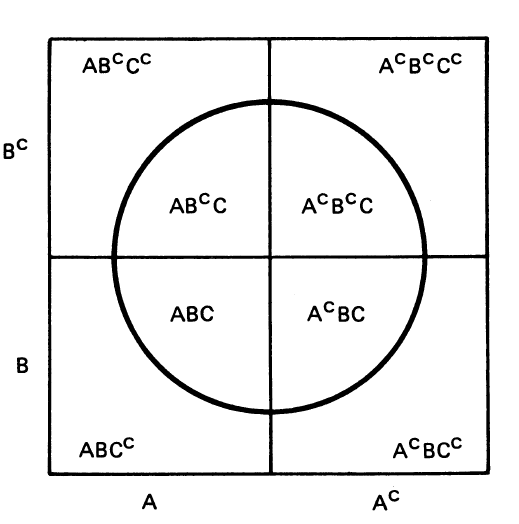
\includegraphics[scale=0.5]{image//Probabilite//1}
\end{wrapfigure}


\chapter{Relations and Operations}
A relation $R$ on $X$ is reflexive if $xRx$ for all $x\in X$,that is,if $R$ contains the $\mathbf{diagonal}$
$$
\bigtriangleup_{X} :=\left \{ (x,x);x\in X \right \}
$$




\chapter{Groups and Homomorphisms}
\section{Cosets}
Let $N$ be a subgroup of G
and $g\in G$.Then $g\odot N$ is the \textbf{left coset} and $N\odot g$ is the \textbf{right coset} of $g\in G$ with respect to $N$ .If we define
$$
g\sim h:\Longleftrightarrow g\in h\odot N
,$$
then $\sim$ is an equivalent relation on $G$:
\textbf{If $\mathbf{g\in h\odot N}$, then there is some $\mathbf{n\in N}$ with $\mathbf{g=h\odot n}$}. Indeed, $\sim$ is reflexive because $e\in N$($g=g\odot e$, 所以$g\sim g$). If $g\in h\odot N$ and $h\in k\odot N$,then
$$
g\in (k\odot N)\odot N=k\odot (N\odot N)=k\odot N
$$




\chapter{Généralité sur espace vectoriel}
\begin{dfn}
        Soient E un ensemble et $\mathbb{K}$ un corps commutatif(ici,$\mathbb{K}=\mathbb{R}$ ou $\mathbb{K}=\mathbb{C}$).On dit que E est un espace vectoriel sur $\mathbb{K}$
(ou bien un $\mathbb{K}$-espace vectoriel)
lorsque E est muni:

-d'une loi de composition interne, notée +,telle que $(E,+)$ soit un group abélien

-d'une loi de omposition externe ,notée $\cdot$, $\cdot$ : $\mathbb{K}\times E \rightarrow E$ vérifiant les propriétés suivantes:

$\bf P1$ $\forall \lambda,\mu \in \mathbb{K},\forall u\in E ,(\lambda+\mu)\cdot u=\lambda\cdot u+\mu\cdot u$

$\bf P2$ $\forall \lambda,\forall u,v\in E ,\lambda\cdot(u+v)=\lambda\cdot u+\lambda\cdot v$


$\bf P3$ $\forall \lambda,\mu \in \mathbb{K},\forall u\in E ,(\lambda\times\mu)\cdot u=\lambda\cdot(\mu\cdot u)$

$\bf P4$ $\forall u\in E ,1_{\mathbb{K}}\cdot u=u$

Les éléments de E sont appelés les vecteurs et les éléments de $\mathbb{K}$ les scalaires
\end{dfn}
\begin{rem}
$(\mathbb{K}^n,+,\cdot)$ est un $\mathbb{K}$-espace vectoriel
\end{rem}
\begin{prp}
        Soit X est un ensemble {\color{red}quelconque} et (F,+,$\cdot$) un $\mathbb{K}$-espace vectoriel.Alors l'ensemble $\mathcal{F}(X,F)$ est un $\mathbb{K}$-espace vectoriel pour les opérations suivantes définies pour tout f,g $\in$ $\mathcal{F}(X,F)$ et $\lambda\in \mathbb{K}$:
\begin{alignat*}{2}
        f\oplus g: X&\rightarrow F&\qquad et \quad \lambda\odot f: X&\rightarrow F\\&x\mapsto f(x)+g(x)
&\quad &x\mapsto \lambda\cdot f(x)
        \end{alignat*}
\end{prp}
\begin{rem}
        Les ensembles $\mathbb{R}^{\mathbb{N}}$,
$\mathbb{R}^{\mathbb{R}}$ et $\mathcal{F}(I,\mathbb{R})$ sont des $\mathbb{R}$-espace vectoriel.Les ensembles $\mathbb{C}^{\mathbb{N}}$,
$\mathbb{C}^{\color{red}\mathbb{R}}$ et $\mathcal{F}(I,\mathbb{C})$ sont des $\mathbb{C}$-espace vectoriel.
\end{rem}
\textbf{之所以给出这些常见的espace vectoriel,是因为我们以后不想再来重复造轮子了,争取一次证明,以后一直用着.}

\begin{rem}
Notez la différence fondamentale dans les règles entre espaces vectoriels et anneaux:

dans un espace vectoriel, $\lambda\cdot u=0\Leftrightarrow  \lambda=0 \quad ou \quad u=0$
\begin{proof}
        $(\lambda\cdot u=0_{E}\Rightarrow \lambda=0_{\mathbb{K}}\quad ou\quad u=0_{E} )\Leftrightarrow(\lambda\cdot u=0_{E}\quad et \quad \lambda\not =0_{\mathbb{K}}\Rightarrow u=0_{E} )$

\textbf{这里用逻辑符号改写,利用同种符号的交换性和否定的改写可以得到这个等价,这样我们就控制了变量。}

        Soient $\lambda$ un scalaire non nul et u un vecteur tels que $\lambda\cdot u=0_{E}$.$\mathbb{K}$ est un corps et $\lambda \not=0_{\mathbb{K}}$ donc $\lambda$ admet un inverse pour la loi $\times$ dans $\mathbb{K}$
Il vient alors:
$$
0_{E}=\lambda^{-1}\cdot 0_{E}=
\lambda^{-1}\cdot(\lambda\cdot u)=(\lambda^{-1}\times\lambda)
\cdot u=1_{\mathbb{K}}\cdot u=u
$$
\end{proof}





dans un anneau,$a\times b=0\not \Rightarrow a=0 \quad ou \quad b=0$
(例子:在($\mathcal{F}(\mathbb{R},\mathbb{R})$,+,$\circ$)这个anneau中定义f和g分别在不同的点不为0,在其他点都为0,则f$\circ$g=0但f$\not$=0且g$\not$=0)
\end{rem}
\begin{dfn}
Soient $u_1,\dots,u_n$ des vecteurs.On appelle combinaison linéaire des vecteurs $u_1,\dots,u_n$ tout
vecteur v sécrivant sous la forme :
$$
v=\sum_{k=1}^{n}\lambda_k\cdot u_k
$$
où $\lambda_1,\dots,\lambda_n$
sont scalaires



\end{dfn}











\begin{dfn}
        Soient E un $\mathbb{K}$-espace vectoriel et F$\subset$E.On dit que F est un sous-$\mathbb{K}$-espace vectoriel de E si:

        (i)$0_{E}\in F$

        (ii)F est stable par combinaisons linéaires
\end{dfn}


\begin{dfn}
        Soient E un espace vectoriel et u un vecteur non nul.On pose alors:
        $$
        \mathbb{K}\cdot u=\left \{ \lambda\cdot u, \lambda\in \mathbb{K} \right \}
        $$
        On dit que $\mathbb{K}\cdot u$ est la droite vectorielle dirigée par u ou que u est un vecteur dircteur de $\mathbb{K}\cdot u$
\end{dfn}
\begin{prp}
        Soit u$\in E\setminus{\{ 0_E\}}$.Alors,    $\mathbb{K}\cdot u$ est un sous-espace vectoriel de E.De plus, tout élément non nul de $\mathbb{K}\cdot u$ est un vecteur directeur de $\mathbb{K}\cdot u$.
\end{prp}






















\chapter{Opération sur les espaces vectoriels}
\section{Intersection et sous-espace engendré par une partie}

\begin{prp}{\bf Intersection}
   Soient E est un $\mathbb{K}$-espace vectoriel et $(F_i)_{i \in I}$ une famille quelconque de sous-espaces vectoriels de E.Alors  $\bigcap_{i \in I}F_{i}$ est un sous-espace vectoriel de E.

\textbf{注意这是一个关于运算的命题,这个运算的被拿出来说的重要性就在这里体现了,也就是子向量空间的交集运算是stable的。}
\end{prp}

\begin{proof}
        On applique les définitions.

        -Pour tout i$\in$I,$F_i$ est un sous-espace vectoriel de E donc:
        $$
        \forall i\in I,0_E\in F_i
        $$
        Ce qui équivaut à $0_E\in\bigcap_{i\in I}F_i$

        -Soient $\lambda,\mu\in \mathbb{K}$ et $u,v \in\bigcap_{i\in I}F_i$.Soit $i \in I$.Puisque $F_i$ est un sous-espace vectoriel de E,$\lambda\cdot u+\mu\cdot v\in F_i$.Ceci étant vrai pour tout $i\in I$,on en déduit que :
$$
\lambda\cdot u+\mu\cdot v\in\bigcap_{i\in I}F_i
$$

Ce qui prouve que $\bigcap_{i\in I}F_i$  est bien un sous-espace vectoriel de E.
\end{proof}










\begin{dfn}{\bf Espace vectoriel engendré par une partie}
Soient E est un $\mathbb{K}$-espace vectoriel et X$\subset$E une partie {\color{red} quelconque} de E.On appelle espace vectoriel
engendré par X,et on note $\mathit{Vect}(X)$
ou $\left \langle X \right \rangle$,l'ensemble défini par :
 \begin{align*}
 \left \langle X \right \rangle = \bigcap_{X\subset F   \atop F sev E}F
 \end{align*}
\end{dfn}

Dans le dessin suivant, on suppose qu'il y a trois sev de E qui contiennent X.(En fait, cette situation ne peut pas se produire en réalité.)
 \begin{figure}[H]
        \centering
        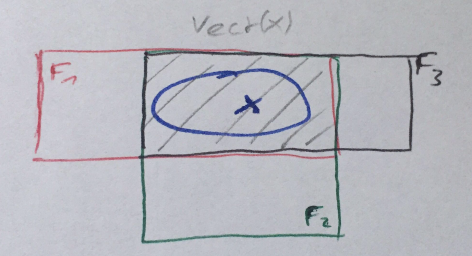
\includegraphics[width=1\textwidth]{image//Operation sur les espaces vectoriels//1}
        \end{figure}

\textbf{注意联系:首先,“叫响名字”:一个是子向量空间的交集运算,一个是从向量空间集E中提取了一个任意子集X来对交集运算中未明的I集合进行抽象的效果定义,即,$I=\left \{i|\quad  X \subset F_i\right \}$, 其实是相当于交集运算中的特例.}

\begin{prp}
        Pour toute partie X$\subset$E,$<X>$ est un sous-espace vectoriel de E et c'est le plus petit sous-espace vextoriel de E(au sens de l'inclusion) qui contient X
\end{prp}
\begin{rem}
        $<\emptyset>=\{0_E\}$
\end{rem}























\section{Somme de sous-espaces vectoriels}
\begin{dfn}{\bf Somme de deux sous-espaces vectoriels }
Soit E un $\mathbb{K}$-espace vectoriel et soient F et G deux sous-espaces vectoriels de E.On définit la somme de F et G, noté $F+G$,
par :
$$F+G=\left \{ u\in E |\quad \exists (x,y)\in F\times G,u=x+y \right \} $$
\end{dfn}
\begin{prp}{\bf Propriété de somme de deux sous-espaces vectoriels}
Avec les hypothèse de la définition , $F+G$ est un sous-espace vectoriel  de contenant F et G, c'est-à-dire que
$$F+G=Vect(F\cup G)$$
\end{prp}
\begin{proof}
        Montrons directement que
        $ F+G=Vect(F\cup G)$,ce qui prouvera également que $F+G$
        est un sous-espace vectoriel de
        E.


        Montrons que $ F+G\subset Vect(F\cup G)$.
        \\
        Soit u $\in F+G$.Par définition , il existe x$\in$F et y$\in$ G tels que u=x+y.On a alors $u=1_\mathbb{K}\cdot x+1_\mathbb{K}\cdot y$ avec x,y $\in$ F$\cup$G et $1_\mathbb{K} \in \mathbb{K}$ donc $u\in \left \langle F\cup G \right \rangle$


        Montrons que $\left \langle F\cup G \right \rangle \subset F+G$
\\
Soit u$\in$	$\left \langle F\cup G \right \rangle$.Il existe $n\in \mathbb{N}, (n)_{0\leq i\leq n}\in
(F+G)^{n+1}$ et $(\lambda_i)_{0\leq i\leq n}\in
\mathbb{K}^{n+1}$ tels que: $u=\sum_{i=0}^{n} \lambda_i x_i$
Posons $I=\left \{ i\in \llbracket 0, n \rrbracket |\quad  x_i\in F \right \}$ et $J= \llbracket 0, n \rrbracket \backslash I$.On a alors
:
$$
u=\sum_{i\in I}\lambda_i x_i\quad+\quad \sum_{j\in J}\lambda_j x_j
$$
Pour tout $i \in I$, $x_i \in F$ et $F$ est un sous-espace vectoriel de $E$ donc: $x=\sum_{i\in I}\lambda_i x_i \in F$.De même, pour tout $j \in J, x_j\in G\backslash F \subset G$
et $G$ est un sous-espace vectoriel
de $E$ donc $y=\sum_{j\in J}\lambda_j x_j \in G
$ .Notez bien que si $I=\emptyset$ ou $J=\emptyset$, le résultat est encore valable puisque $\sum_{i\in \emptyset}\lambda_i x_i=0_E$ qui appartient bien à $F$ et à $G$
.

Ainsi,$u=x+y$ avec $x \in F$  et $x \in G$, c'est-à-dire $u \in F+G$. D'où , la seconde inclusion
\end{proof}

\section{Sommes directes et sous-espaces sectoriels supplémentaires}

\paragraph{Proposition: 直和的等价(具体形式)}
Soient E un $\mathbb{K}$-espace vectoriel et F,G deux sous-espaces vectoriels de E.Alors les propriétés suivantes sont équivalentes:

($i$)F et G sont en somme dircte;

($ii$)Tout éléments u de $F+G$ se décompense de façon unique sous la forme $u-x+y$ avec $x\in F$ et $y\in G$,c'est-à-dire $$\forall u\in F+G, \exists!(x,y)\in F\times G, u=x+y$$
\begin{proof}
        Montrons $(ii)\implies(i)$.
\\
On suppose $(ii)$.Soit $x\in F\cup G$.Alors, par exemple,$(-x)\in G$.Il s'ensuit que $0_E=x+(-x)$ avec $x\in F$ et $(-x)\in G$.Or, on a également $0_E\in F\cup G$ : on peut donc aussi écrire $0_E=0_E+0_E$ avec $(0_E,0_E)\in F\times G$.D'aprês $(ii)$, la décomposition est unique :
ceci implique que $x=0_E$,prouvant ainsi que $F\cup G={0_E}$
\end{proof}
\paragraph{Definition: Supplémentaire}
Soient E un $\mathbb{K}$-espace vectoriel et $F,G$ deux sous-espace vectoriels de E.On dit que $F$ et $G$ sont supplémentaires (ou supplémentaire dans E) si tout vecteur de E peut se décomposer de façon unique en la somme d'un vecteur de F et d'un vecteur de G.Autrement dit $F$ et $G$ sont supplémentaire si:
$$
\forall u\in F+G, \exists!(x,y)\in F\times G, u=x+y
$$

\paragraph{Théorème: Existence du supplémentaire}
Soit E un espace sectoriel et soit F un sous-espace vectoriel de E. Alors F admet au moins un supplémentaire dans E.

\section{Produit cartésien de deux espaces vectoriel}

\chapter{Applications linéaires}
\begin{dfn}{\bf Applications Linéaires}
morphisme
\end{dfn}

\begin{prp}
{\bf Equivalence pour voir si une application  est linéaire}
\textbf{验证线性映射的过程,有一点像验证子向量空间的线性组合stable的过程(区别在于原来是在一个集合内部,现在是两个集合之间),但是因为线性映射的定义的性质中带有$\mathbf{f(0_E)=0_F}$,所以不用看}

\textbf{这个命题还是比较有意思的,有助于理解线性映射的定义和外延.注意如何在未知是线性映射的情况下要重新证明$\mathbf{f(0_E)=0_F}$}

$\mathbf{f:\mathbb{R}^2\longrightarrow \mathbb{R}^2,\quad (x,y)\longmapsto (2x,x+y)} $
\textbf{比较抽象的线性映射}

否定一个线性映射可以用$f(0_E)\neq 0_F$来判断
\end{prp}

\paragraph{Définition: forme linéaire}





\subsection{Restriction et recollement}
\begin{thm}{\bf Théorème de recollement}  Soient E,F deux $\mathbb{K}$-espaces vectoriels et G,H deux sous-espaces vectoriels supplémentaire dan E.Alors l'application:
\begin{align*}
\phi:\mathcal{L}(E,F)\rightarrow \mathcal{L}(G,F)\times \mathcal{L}(H,F)\\
f\mapsto (f|_{G},f|_{H})
\end{align*}
est un isomorphisme de $\mathbb{K}$-espaces vectoriels.En clair ,la connaissance d'une application linéaire sur deux sous-espaces  vectoriels supplémentaire détermine l'application linéaire de façon unique.
\end{thm}
\begin{proof}
        \begin{itemize}


\item Tout d'abord,d'après ce qui précède ,$\mathcal{L}(E,F),\mathcal{L}(G,F),\mathcal{L}(H,F)$ sont des $\mathbb{K}$-espace vectoriel.Par suite,$\mathcal{L}(G,F)\times\mathcal{L}(H,F)$ est aussi un
$\mathbb{K}$-espace vectoriel.
\item Ensuite,d'après la proposition précédente,si $f\in\mathcal{L}(E,F)$,alors $f_{|G}\in\mathcal{L}(G,F)$
et $f_{|H}\in\mathcal{L}(H,F)$.Par conséquent,$\phi$ est bien définie.
\item Par ailleurs, il est clair que pour toutes $f,g\in
\mathcal{L}(E,F)$,pour tout $\lambda,\mu\in\mathbb{K}$,et pour tout sous-espace vectoriel A de E,$(\lambda\cdot f+\mu\cdot g)
_{|A}=\lambda\cdot f_{|A}+\mu\cdot g_{|A}$.
Par suite,$\phi$ est linéaire.
\item Montrons enfin que $\phi$ est bijective.

-Injectivité

Soit $f\in ker\phi$.Montrons que $f=0$.Par définition de $\phi$,$f_{|G}=0$ et $f_{|H}=0$.Soit alors $x\in E$
Puisque G et H sont supplémentaires dans E,il existe un unique couple (a,b)$\in G\times H$ tel que $x=a+b$.On a alors :

\begin{alignat*}{5}
    f(x)&=f(a+b)\\
    &=f(a)+f(b)\\
    &=f_{|G}(a)+f_{|H}(b)\\
    &=0+0\\
    &=0
\end{alignat*}
Par conséquant,pour tout $x\in E,f(x)=0$,c'est-à-dire $f=0$(application nulle) et $ker\phi=\{0\}$,c'est-à-dire $\phi$ est injective.

-Surjectivité

Soient g$\in \mathcal{L}(G,F)$ et h$\in \mathcal{L}(H,F)$,Montrons qu'il existe $f\in \mathcal{L}(E,F)$ telle que
$f_{|G}\in\mathcal{L}(G,F)$
et $f_{|H}\in\mathcal{L}(H,F)$.

Soit $x\in E$:il exist un unique couple $(a,b)\in G\times H$ tel que $x=a+b$.On pose alors $f(x)=g(a)+h(b)$.Ceci définit bien une application $f$ de E dans F puisque le couple (a,b)
est unique.Montrons alors que
$f$ convient.
\begin{itemize}
 \item Si $x\in G$,alors par unicité du couple $(a,b)\in G\times H$ tel que $x=a+b$,on a $a=x$ et $b=0$.Alors,$f(x)=g(a)+h(b)=g(x)+h(0)=g(x)+0=g(x)$.Par suite,$f_{|G}=g$.
 \item De la même façon,on montre que $f_{|H}=h$.
 \item Montrons enfin que $f\in\mathcal{L}(E,F)$.

 Soient $x,x'\in E$ et $\lambda \in \mathbb{K}$.
 Il existe alors un unique couple $(a,b)\in G\times H$ et un unique couple $(a,b)\in G\times H$ tels que $x=a+b$ et $x'=a'+b'$.On a alors $\lambda \cdot x+x'=(\lambda\cdot a+a')+(\lambda\cdot b+b')$.G et H étant des sous-espaces vectoriels de E,$ (\lambda\cdot a+a',\lambda\cdot b+b')\in G\times H$,Par suite,
 \begin{alignat*}{4}
 f(\lambda\cdot x+x')&=g(\lambda\cdot a+a')+h(\lambda\cdot b+b')\\
 &=\lambda \cdot g(a)+g(a')+\lambda\cdot h(b)+h(b')\\
 &=\lambda\cdot(g(a)+h(b))+g(a')+h(b')\\
 &=\lambda\cdot f(x)+f(x')
 \end{alignat*}
 Ce qui prouve que $f$ est une application linéaire.
\end{itemize}
\end{itemize}
Ainsi,on a montre que pour tout $(g,h)\in \mathcal{L}(G,F)\times \mathcal{L}(H,F)$ qu'il existe $f\in \mathcal{L}(E,F)$ telle que
$f_{|G}\in\mathcal{L}(G,F)$
et $f_{|H}\in\mathcal{L}(H,F)$,c'est-à-dire $\phi(f)=(g,h)$.Par conséquant,$\phi$ est surjective.

\end{proof}

\chapter{Eigenvalues and Eigenvectors}
\section{Invariant Subspaces}
In this chapter we develop the tools that will help us understand the structure of operators. Recall that an operator is a linear map from a vector space to itself. Recall also that we denote the set of operators on $V$ by $\mathcal{L}(V) ;$ in other words, $\mathcal{L}(V)=\mathcal{L}(V, V)$.

Let's see how we might better understand what an operator looks like. Suppose $T \in \mathcal{L}(V)$. If we have a direct sum decomposition
\begin{equation}
V=U_{1} \oplus \cdots \oplus U_{m},\label{1}
\end{equation}
where each $U_{j}$ is a proper subspace of $V$, then to understand the behavior of $T$, we need only understand the behavior of each $\left.T\right|_{U_{j}}$; here $\left.T\right|_{U_{j}}$ denotes the restriction of $T$ to the smaller domain $U_{j} .$ Dealing with $\left.T\right|_{U_{j}}$ should be easier than dealing with $T$ because $U_{j}$ is a smaller vector space than $V$. However, if we intend to apply tools useful in the study of operators (such as taking powers), then we have a problem:
$\left.T\right|_{U_{j}}$ may not map $U_{j}$ into itself; in other words, $\left.T\right|_{U_{j}}$ may not be an operator on $U_{j}$. Thus we are led to consider only decompositions of the form $\ref{1}$ where $T$ maps each $U_{j}$ into itself.

The notion of a subspace that gets mapped into itself is sufficiently important to deserve a name. Thus, for $T \in \mathcal{L}(V)$ and $U$ a subspace of $V,$ we say that $U$ is \textbf{invariant} under $T$ if $u \in U$ implies $T u \in U$. In other words, $U$ is invariant under $T$ if $\left.T\right|_{U}$ is an operator on $U$. For example, if $T$ is the operator of differentiation on $\mathcal{P}_{7}(\mathbf{R})$, then $\mathcal{P}_{4}(\mathbf{R})$ (which is a subspace of $\left.\mathcal{P}_{7}(\mathbf{R})\right)$ is invariant under $T$ because the derivative of any polynomial of degree at most 4 is also a polynomial with degree at most 4.

Let's look at some easy examples of invariant subspaces. Suppose $T \in \mathcal{L}(V)$. Clearly \{0\} is invariant under $T$. Also, the whole space $V$ is obviously invariant under $T$. Must $T$ have any invariant subspaces other than \{0\} and $V ?$ Later we will see that this question has an affirmative answer for operators on complex vector spaces with dimension greater than 1 and also for operators on real vector spaces with dimension greater than 2.

If $T \in \mathcal{L}(V),$ then null $T$ is invariant under $T$ (proof: if $u \in \operatorname{null} T$, then $T u=0$, and hence $T u \in$ null $T$ ). Also, range $T$ is invariant under $T$ (proof: if $u \in$ range $T$, then $T u$ is also in range $T$, by the definition of range). Although null $T$ and range $T$ are invariant under $T$, they do not necessarily provide easy answers to the question about the existence of invariant subspaces other than \{0\} and $V$ because null $T$ may equal \{0\} and range $T$ may equal $V$ (this happens when $T$ is invertible).

We will return later to a deeper study of invariant subspaces. Now we turn to an investigation of the simplest possible nontrivial invariant subspaces-invariant subspaces with dimension $1 .$

How does an operator behave on an invariant subspace of dimension $1 ?$ Subspaces of $V$ of dimension 1 are easy to describe. Take any nonzero vector $u \in V$ and let $U$ equal the set of all scalar multiples of $u$ :
\begin{equation}
U=\{a u: a \in \mathbf{F}\}\label{2} .
\end{equation}
Then $U$ is a one-dimensional subspace of $V$, and every one-dimensional subspace of $V$ is of this form. If $u \in V$ and the subspace $U$ defined by $\ref{2}$ is invariant under $T \in \mathcal{L}(V),$ then $T u$ must be in $U,$ and hence there must be a scalar $\lambda \in \mathbf{F}$ such that $T u=\lambda u .$ Conversely, if $u$ is a nonzero vector in $V$ such that $T u=\lambda u$ for some $\lambda \in \mathbf{F}$, then the subspace $U$ defined by $\ref{2}$ is a one-dimensional subspace of $V$ invariant under $T$.

The equation
\begin{equation}
T u=\lambda u\label{3}
\end{equation}
which we have just seen is intimately connected with one-dimensional invariant subspaces, is important enough that the vectors $u$ and scalars $\lambda$ satisfying it are given special names. Specifically, a scalar $\lambda \in \mathbf{F}$ is called an \textbf{eigenvalue} of $T \in \mathcal{L}(V)$ if there exists a nonzero vector $u \in V$ such that $T u=\lambda u .$ We must require $u$ to be nonzero because with $u=0$ every scalar $\lambda \in \mathbf{F}$ satisfies $\ref{3}.$ The comments above show that $T$ has a one-dimensional invariant subspace if and only if $T$ has an eigenvalue.

The equation $T u=\lambda u$ is equivalent to $(T-\lambda I) u=0,$ so $\lambda$ is an eigenvalue of $T$ if and only if $T-\lambda I$ is not injective.$\lambda$ is an eigenvalue of $T$ if and only if $T-\lambda I$ is not invertible, and this happens if and only if $T-\lambda I$ is not surjective.

Suppose $T \in \mathcal{L}(V)$ and $\lambda \in \mathbf{F}$ is an eigenvalue of $T .$ A vector $u \in V$ is called an eigenvector of $T$ (corresponding to $\lambda$ ) if $T u=\lambda u$. Because $\ref{3}$ is equivalent to $(T-\lambda I) u=0$, we see that the set of eigenvectors of $T$ corresponding to $\lambda$ equals $\operatorname{null}(T-\lambda I) .$ In particular, the set of eigenvectors of $T$ corresponding to $\lambda$ is a subspace of $V$.

Let's look at some examples of eigenvalues and eigenvectors. If $a \in \mathbf{F}$, then $a I$ has only one eigenvalue, namely, $a$, and every vector is an eigenvector for this eigenvalue.

For a more complicated example, consider the operator $T \in \mathcal{L}\left(\mathbf{F}^{2}\right)$ defined by
\begin{equation}
T(w, z)=(-z, w)\label{4}
\end{equation}
If $\mathbf{F}=\mathbf{R}$, then this operator has a nice geometric interpretation: $T$ is just a counterclockwise rotation by $90^{\circ}$ about the origin in $\mathbf{R}^{2} .$ An operator has an eigenvalue if and only if there exists a nonzero vector in its domain that gets sent by the operator to a scalar multiple of itself. The rotation of a nonzero vector in $\mathbf{R}^{2}$ obviously never equals a scalar multiple of itself. Conclusion: if $\mathbf{F}=\mathbf{R}$, the operator $T$ defined by $\ref{4}$
has no eigenvalues. However, if $\mathbf{F}=\mathbf{C},$ the story changes. To find eigenvalues of $T$, we must find the scalars $\lambda$ such that
$$
T(w, z)=\lambda(w, z)
$$
has some solution other than $w=z=0$. For $T$ defined by $\ref{4}$ , the equation above is equivalent to the simultaneous equations
\begin{equation}
-z=\lambda w, \quad w=\lambda z\label{5}
\end{equation}

Substituting the value for $w$ given by the second equation into the first equation gives $-z=\lambda^{2} z$
Now $z$ cannot equal 0 (otherwise $\ref{5}$ implies that $w=0$; we are looking for solutions to $\ref{5}$ where $(w, z)$ is not the 0 vector), so the equation above leads to the equation
$$
-1=\lambda^{2}
$$
The solutions to this equation are $\lambda=i$ or $\lambda=-i$. You should be able to verify easily that $i$ and $-i$ are eigenvalues of $T .$ Indeed, the eigenvectors corresponding to the eigenvalue $i$ are the vectors of the form $(w,-w i)$, with $w \in \mathbf{C}$, and the eigenvectors corresponding to the eigenvalue $-i$ are the vectors of the form $(w, w i),$ with $w \in \mathbf{C}.$




\chapter{Polynômes}
\section{Théorème d'aporoximation de Weierstrass à l'aide des polynômes de Bernstein}
\begin{thm}[Théorème d'approximation de Weierstrass]
Toute fonction continue sur [0,1] est limite uniforme de fonctions polynomiales. 
\end{thm}
\begin{proof}
下面我们借助于伯恩斯坦多项式分几步来证明它:

Dans toute la discussion, on identifiera un polynôme et sa fonction polynomiale associée.

Soit  $f: [0.1] \rightarrow \mathbb{R}$ une application continue. Pour n $\in \mathbb N ^{*}$ , on définie le $n^{\text{ième}}$  polynôme de Bernstein associé à f par:

​$$\boxed{B_{n}(f)(x) = \sum_{k=0}^{n}\binom{n}{k}f(\frac{k}{n})x^k(1-x)^{n-k}}$$ 

Soit $\epsilon > 0$ .D'aprè le théoreme de Heine, il existe $\eta > 0$ tel que pour $(x,y) \in [0,1]^2$ . si $\left | x-y \right | \le\eta$  alors       $\left | f(x)-f(y) \right | \le\frac{\epsilon}{2}.$  

On note $M$  la borne supérieure de $\{\left |f(x)\right| / x\in [0,1]\}$ .On se fixe $x\in [0,1]$ .


1.Montrer que 

​ $$f(x)-B_{n}(f)(x) = \sum_{k=0}^{n}\binom{n}{k}(f(x)-f(\frac{k}{n}))x^k(1-x)^{n-k}.$$



2.(a)Montrer que

$$\sum_{0\le k\le n, \left | x-\frac{k}{n} \right | \color{blue}{\le}\eta}\binom{n}{k}\left|(f(x)-f(\frac{k}{n}))\right|x^k(1-x)^{n-k}\le\frac{\epsilon}{2}.$$ 

​2.(b)Montrer que 

$$\sum_{0\le k\le n, \left | x-\frac{k}{n} \right | \color{red}{>}\eta}\binom{n}{k}\left|(f(x)-f(\frac{k}{n}))\right|x^k(1-x)^{n-k}\le\frac{2M}{\eta^2}\sum_{k=0}^{n}\binom{n}{k}(x-\frac{k}{n})^2x^k(1-x)^{n-k}$$



3.Calculer $B_{n}(t\mapsto t)(x)$ et $B_{n}(t\mapsto t^2)(x)$.On pourra introduire $S:  y\mapsto (y+1-x)^n$ .

(difficile,提示:利用好新引入的变量y与x的区别,试试展开S以及对分别对展开前后的S关于y求导,比照与要计算式子的区别并乘上缺的x幂次)

4.Montrer que 

$$\sum_{0\le k\le n, \left | x-\frac{k}{n} \right | \color{red}{>}\eta}\binom{n}{k}\left|(f(x)-f(\frac{k}{n}))\right|x^k(1-x)^{n-k}\le\frac{M}{2\eta^2 n}.$$

(difficle+,要利用2(b)和3中的结论,试着展开2(b)不等式右边的$(x-k/n)^2$项,并试着代入3中求得的两个式子)

5.Prouver que pour $\epsilon>0$ ,il existe $N\in \mathbb N$ tel que pour $x\in [0,1],\left|f(x)-B_{n}(f)(x)\right|\le \epsilon.$

(difficile+,注意这里是对整个的$x\in[0,1]$ ,利用2(a)和4中的结论)

On dit que f est approchée uniformément sur [0,1] par les polynomes $B_{n}(f)$.
\end{proof}





\chapter{Integration}
We now turn to integration, which we develop as the ‘area under the curve’. We establish the existence and properties of the Riemann integral; this is an integral whose development is quite straightforward, and which is good for many of the needs of analysis. It has some shortcomings: it can only be applied to a restricted class of functions, and it is not easy to obtain good results about limits of integrals. For this, a more sophisticated(复杂的) integral, the Lebesgue integral, is needed.

As with all theories of integration, we proceed by approximation. To
begin with, we restrict attention to bounded real-valued functions on
a finite interval $[a, b].$ The easiest functions to start with are
the step functions —— functions which take constant values $v_j$ on a
finite set $\left\{I_j : 1 \le j \le k\right\}$ of disjoint
sub-intervals of $[a, b].$ The graph of such a function is a bar
graph, and we define the elementary integral of such a function to be
$\sum^k_{j=1} v_jl(I_j),$ where $l(I_j)$ is the length of the interval
$I_j.$ Note that $v_j$ can be positive or negative, so that the
integral can take positive and negative values. The idea of the
Riemann integral of a function $f$ is to approximate $f$ from above
and below by step functions. If the integrals of the approximations
from above and from below approach a common limit, then we take this
limit to be the Riemann integral of $f.$ In order to carry out this
programme, we need to set up the appropriate machinery. A
{\bf{dissection}} $D$ of $[a, b]$ is a {\bf finite subset} of $[a, b]$ which contains both $a$ and $b.$ We arrange the elements of $D,$ the points of dissection of $D,$ in increasing order: $a = x_0 < x_1 < \cdots < x_k = b.$ The dissection splits $[a, b]$ into $k$ disjoint intervals $I_1,\cdots I_k.$ We need to decide what to do with the endpoints; we adopt the convention that $I_1 = [x_0, x_1]$ and that $I_j = (x_{j−1}, x_j ]$ for $2 \le j<k.$
We order the dissections of $[a, b]$ by inclusion: we say that $D_2$ {\bf{refines}} $D_1$ if $D_1 \subset D_2,$ and write $D_1 \le D_2.$ This is a partial order on the set $\Delta$ of all dissections of $[a, b],$ and $\Delta$ is a lattice: $D_1\vee D_2 = D_1 \cup D_2$ and $D_1 \wedge D_2 = D_1 \cap D_2.$ $\Delta$ has a least element $\left\{a, b\right\},$ but has no greatest element.
Suppose that $D$ is a dissection, with intervals $I_1,\cdots,I_k.$ We denote the indicator function of $I_j$ by $\chi_j$ : $\chi_j (x) = 1$ if $x \in I_j,$ and $\chi_j (x) = 0$ otherwise. Similarly, we write $\chi_{[a,b]}$ for the indicator function of $[a, b].$ We denote the linear span of $\left\{\chi_j : 1 \le j \le k\right\}$ by $E_D;$ thus a function $f \in E_D$ is of the form $f =\sum^k _{j=1} v_j\chi_j ,$ where $v_1,\cdots,v_k$ are real numbers. The elements of $E_D$ are the step functions on $[a, b]$ whose points of discontinuity are contained in $D;$ note that, according to our convention, step functions are continuous on the left. $E_D$ is a $k$-dimensional vector space of functions. If $D_2$ refines $D_1,$ then $E_{D_1} \subset E_{D_2},$ and so the set of spaces $\left\{E_D : D \in \Delta\right\}$ also forms a lattice:
$$
\begin{aligned}
  E_{D_{1}} & \wedge E_{D_{2}}=E_{D_{1}} \cap E_{D_{2}}=E_{D_{1} \wedge D_{2}}
\end{aligned}
$$
and
$$
\begin{aligned}
 E_{D_{1}} \vee E_{D_{2}} &=\operatorname{span}\left(E_{D_{1}} \cup E_{D_{2}}\right)=E_{D_{1} \vee D_{2}}
\end{aligned}
$$
The union $E_{\Delta}=\cup\left\{E_{D}: D \in \Delta\right\}$ is the infinite-dimensional vector space of all (left-continuous) step functions.
We now wish to define the elementary integral of a step function $f .$ If $f=\sum_{j=1}^{k} v_{j} \chi_{j},$ we want to define $\int_{a}^{b} f(x) d x$ to be $\sum_{j=1}^{k} v_{j} l\left(I_{j}\right),$ where $l\left(I_{j}\right)=x_{j}-x_{j-1}$ is the length of $I_{j} .$ But the representation is not unique, and we need to show that the integral is well-defined.
\begin{prp}
  Suppose that $D$ and $D'$ are dissections of $[a, b],$ and that $f \in E_D\cap E_D' ,$ with representations $f =\sum^k_{j=1} v_j\chi_j$ and $f =\sum^{k'}_{j=1} v'_j\chi'_j .$ Then $$\sum^k_{j=1}v_jl(I_j)=\sum^{k'}_{j=1} v'_j l(I'_j).$$
\end{prp}
\begin{proof} We use the lattice property of $\Delta.$ Let $D'' = D \cup D'.$ Let $D = \left\{x_0,\cdots,x_k\right\}$ and $D'' = \left\{x''_0,\cdots,x''_{k''}\right\}.$ Then there exist $0 = r_0 < r_1 < \cdots < r_k = k''$ such that $x_j = x''_{r_j}$ for $0 \le j \le k.$ Thus $$l(I_j) =\sum^{r_j}_{r=r_{j−1}+1} l(I''_r).$$ 注意区间是按后一个点的序号算,这里求和的$r$是按1到$k''$的序走,不是按$r_{k}$的角标序(1到$k$)走.We can write $f =\sum^{k''}_{r=1} v''_r\chi''_r,$ where $v_j = v''_r$ for $r_{j−1} < r \le r_j.$ Consequently, $$\sum^k_{j=1}v_j l(I_j) = \sum^k_{j=1} \left( \sum^{r_j}_{r=r_{j−1}+1} v''_r l(I''_r )\right) = \sum^{k''}_{r=1} v''_r l(I''_r).$$
Similarly, $\sum^{k'}_{j=1}v'_j l(I'_j)=\sum^{k''}_{r=1} v''_r l(I''_r)$, so that $$\sum^k_{j=1}v_jl(I_j)=\sum^{k'}_{j=1} v'_j l(I'_j).$$
We can therefore define the elementary integral as $$\int_{a}^{b} f(x) d x=  \sum^k_{j=1}v_jl(I_j).$$
\end{proof}
\begin{rem}
A partially ordered set $(A, \le)$ is called a {\bf{lattice}} if
whenever $a$ and $b$ are elements of $A$ then the set $\left\{a,
  b\right\}$ has an infimum, denoted by $a\wedge b,$ and a supremum,
denoted by $a \vee b.$
\end{rem}
\section{Upper and lower Riemann integrals}
We now consider a bounded function f on [a, b], with $m \le f(x) \le M$ for all
$x \in [a, b].$  We try to integrate it by approximating from above and below by
step functions. Let
$$U_f = \left\{g : g \in E_{\Delta}\text{ and }g \ge f\right\}$$
be the set of step functions which are greater than or equal to $f$. $U_f$ is
non-empty, since $M_{\chi_{[a,b]}} \in U_f$. If $g \in U_f, g \ge m_{\chi_{[a,b]}}$, and so
$\int_{a}^{b}g(x) dx \ge m(b-a)$.Thus the set $\left\{\int^b_a g(x) dx : g \in U_f\right\}$ is bounded below. We define
the {\bf upper Riemann integral} of f to be
$$
\overline{\int^b_a}f(x)d x=\inf\left\{\int^b_a g(x) dx : g \in U_f\right\}
$$
很诡异的定义: 先定义f的“上阶分(阶梯分划)集”,然后给“上阶分集”的定积分集取$\inf$,也就是在
“上阶分集”的定积分集的下界中找一个最大值,即:{\bf 上下上}.上下不在一个范畴内,一
个是阶梯函数集,一个是定积分集.

Similarly we set
$$L_f = \left\{h : h \in E_{\Delta}\text{ and }h \le f\right\}$$
and define the {\bf lower Riemann integral} of f to be
$$
\underline{\int^b_a}f(x)d x=\sup\left\{\int^b_a h(x) dx : h \in L_f\right\}
$$
\begin{prp}
Suppose that $f$ is a bounded function on $[a, b] .$ Then $\underline{\int_{a}^{b}} f(x) d x \leq \overline{\int_{a}^{b}} f(x) d x$
\end{prp}
\begin{proof}
$\quad$ If $h \in L_{f}$ and $g \in U_{f}$ then $h \leq f \leq g,$ so that
$$
\int_{a}^{b} h(x) d x \leq \int_{a}^{b} g(x) d x
$$
Taking the supremum over $L_{f},$ we see that
$$
\underline{\int_{a}^{b}} f(x) d x \leq \int_{a}^{b} g(x) d x,
$$
so that, taking the infimum over $U_{f}$,
$$
\underline{\int_{a}^{b}} f(x) d x \leq \inf \left\{\int_{a}^{b} g(x) d x: g \in U_{f}\right\}=\overline{\int_{a}^{b}} f(x) d x
$$
\end{proof}
Suppose that D is a dissection, with intervals $I_1, \cdots , I_k$, and that f is
a bounded function on [a, b]. Let $M(I_j) =\sup\left\{f(x) : x \in I_j\right\}$, and let
$M_D(f) = \sum^k_{j=1} M_j\chi_j$. Then $M_D(f)$ is the least element of $E_D \cap U_f =\left\{g \in
E_D, g \ge f\right\}$.这时候又对“上阶分集”中的函数取了最小值,但这个最小
值函数又是在对函数值的上集取了最小值的基础上构建的. We set
$$S_D = S_D(f) =\sum^k_{j=1}M(I_j)l(I_j) =\int^b_aM_D(f)(x) d x.$$
这个地方就是难点交汇处,我们要找的是所有“上阶分集”中函数的积分集的下界的最大值,我
们构造了一个对特定划分的“上阶分集”中的函数的最小值,现在需要建立它们之间的联系。
Then $$S_D = \inf\left\{\int^b_a g(x) dx : g \in U_f \cap E_D\right\},$$
对应关系:“上阶分集”中函数的积分集的下界的最大值=“上阶分集”中的最
小值函数的积分.这里简化就是:“下界的最大值”=最小值.这是成立的.因为最小值
是实打实存在的,这是阶梯函数的特殊性,可以类比于整数相对于实数的特殊性.顺
便吐槽一下,这里的困惑全部来源于对$\sup,$$\inf,$$\min,$和$\max$不加证
明的使用,可见法国人的严谨是有必要的,步步为营最后反而赢得时间,
so that
$$\begin{aligned}
\overline{\int^b_a}f(x) dx &=\inf\left\{\inf\left\{
\int^b_ag(x) dx : g \in U_f \cap E_D\right\} : D \in \Delta\right\}\\
&=\inf\left\{S_D : D \in \Delta\right\}.
\end{aligned}$$
Similarly, we define $m(I_j) =\inf\left\{f(x) : x \in I_j\right\}$ and
$m_D(f) = \sum^k_{j=1} m_j(I_j)\chi_j$
and set $$s_D = s_D(f) =\sum^k_{j=1}m(I_j)l(I_j) =\int^b_am_D(f)(x) d x.$$
Then $$s_D = \sup\left\{\sup\int^b_a h(x) dx : h \in L_f \cap E_D\right\},$$ so that
$$\begin{aligned}
\underline{\int^b_a}f(x) dx &=\sup\left\{\sup\left\{
\int^b_ah(x) dx : h \in L_f \cap E_D\right\} : D \in \Delta\right\}\\
&=\sup\left\{s_D : D \in \Delta\right\}.
\end{aligned}$$
\begin{figure}[H]
  \centering
  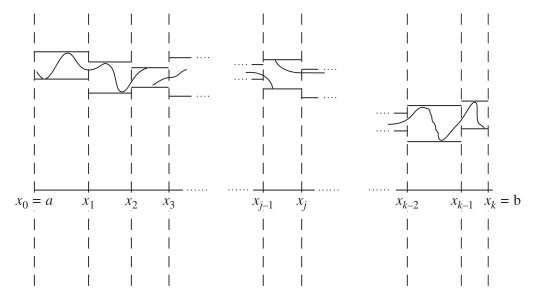
\includegraphics[width=0.8\linewidth]{image//Integration//1}
  \caption{Upper and lower sums $S_D$ and $s_D$.}
\end{figure}
Note that if $D^{\prime}$ refines D then $S_{D^{\prime}} \le S_D$ and $s_{D^{\prime}} \ge s_D$.

In fact, we do not need to consider all the dissections to determine the
upper and lower Riemann integrals. If D is a dissection, with intervals
$I_1, \cdots, I_k$, we define the {\bf mesh size} $\delta(D)$ to be $\max\left\{l(I_j) : 1 \le j \le k\right\}$.

\begin{thm}
Suppose that $(D_r)^{\infty}_{r=1}$ is a sequence of dissections of [a, b],
and that $\delta(D_r) \to 0$ as $r \to \infty$. If f is a bounded function on [a, b] then
$S_{D_r}(f) \to\overline{\int^b_a} f(x) d x$ as $r\to\infty$.
\end{thm}
\begin{proof}
Suppose that $\epsilon > 0$. Then there exists a dissection D of [a, b],
with points of dissection $a = x_0 < x_1 < \cdots < x_k = b$ such that
$S_D <\int^b_a f(x) dx + \epsilon/2.$ The idea of the proof is to choose r large enough so
that the set D is contained in a set of intervals of $D_r$ of small
total length.(这里的D是分点的集合,但我们要求的是$D_r$划分的小区间(每个
小区间的长度都很短)要包含组成D的分点,可以说又一次有点跳脱维度) Let
$\eta = \frac{\epsilon}{2(k + 1)(M − m + 1)}$. There exists $r_0$ such that $\delta(D_r) < \eta$ for $r \ge r_0$.
Suppose that $r \geq r_{0} .$ Let $D^{\prime}=D \vee D_{r} .$ Then $S_{D^{\prime}} \leq S_{D} .$ Let $\left\{J_{1}, \ldots, J_{q}\right\}$
be the intervals of the dissection $D_{r},$ and let $K_{1}, \ldots,
K_{s}$ be the intervals of the dissection $D^{\prime} .$ We divide
$\{1, \ldots, q\}$ into two disjoint subsets. Let $p \in B$ if $J_{p}$
contains one or more elements of $D,$ and let $p \in G$
otherwise. $(B$ is the set of bad indices, and $G$ is the set of good
indices.) Then $|B| \leq k+1$. If $p \in B,$ then $J_{p}$ is the
disjoint union $\cup_{r \in S_{p}} K_{r}$(所有此$J_p$旗下包含的D的
端点把此$J_P$二次分化后,对应到$D^{\prime}$中划分出区间的序号) of finitely many of
intervals in $D^{\prime} .$  Since $m \le f(x) \le M,$
$$M l\left(J_{p}\right) \geq M\left(J_{p}\right) l\left(J_{p}\right) \geq \sum_{r \in S_{p}} M\left(K_{r}\right) l\left(K_{r}\right) \geq m \sum_{r \in S_{p}} l\left(K_{r}\right)=m l\left(J_{p}\right) .
$$
If $p \in G,$ then $J_{p}=K_{r}$ for some $r \in\{1, \ldots, s\},$ so that $M\left(J_{p}\right)=M\left(K_{r}\right)$ Thus
$$
\begin{aligned}
S_{D_{r}}-S_{D^{\prime}} &\left.=\sum_{p \in
    B} \left(M_{p}l\left(J_{p}\right)-\sum_{r \in S_{p}}
    M\left(K_{r}\right) l(K_{r}) \right)\right. \\
& \leq \sum_{p \in B}(M-m) l\left(J_{p}\right) \leq(M-m)(k+1) \delta\left(D_{r}\right)<\epsilon / 2
\end{aligned}
$$
Consequently, if $r \geq r_{0}$ then
$$
\int_{a}^{b} f(x) d x \leq S_{D_{r}} \leq S_{D^{\prime}}+\epsilon / 2 \leq S_{D}+\epsilon / 2<\int_{a}^{b} f(x) d x+\epsilon
$$
so that $S_{D_{r}} \rightarrow \overline{\int_{a}^{b}} f(x) d x$ as $r
\rightarrow \infty$


\end{proof}

\chapter{The Genesis of Fourier Analysis}
\section{The vibrating string}
\subsection{简介}
The problem consists of the study of the motion of a string fixed at its end points and allowed to vibrate freely. We have in mind physical systems such as the strings of a musical instrument. As we mentioned above, we begin with a brief description of several observable physical phenomena on which our study is based. These are:

- simple harmonic motion,

- standing and traveling waves,

- harmonics and superposition of tones.

Understanding the empirical facts behind these phenomena will motivate our mathematical approach to vibrating strings.
\subsubsection{Simple harmonic motion}
Simple harmonic motion describes the behavior of the most basic oscillatory system (called the simple harmonic oscillator), and is therefore a natural place to start the study of vibrations. Consider a mass $\{m\}$ attached to a horizontal spring, which itself is attached to a fixed wall, and assume that the system lies on a frictionless surface.

Choose an axis whose origin coincides with the center of the mass when it is at rest (that is, the spring is neither stretched nor compressed), as shown in $\reffig{p1}$.
\begin{figure}[H]\centering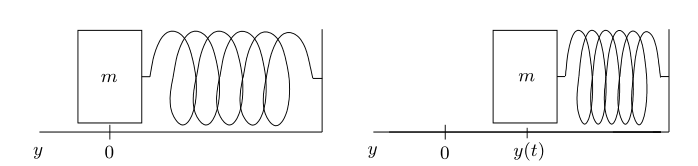
\includegraphics[width=1\textwidth]{image//The Genesis of Fourier Analysis//1}
\caption{Simple harmonic oscillator}
\label{p1}	
\end{figure}
 When the mass is displaced from its initial equilibrium position and then released, it will undergo simple harmonic motion. This motion can be described mathematically once we have found the differential equation that governs the movement of the mass.
 
 Let $y(t)$ denote the displacement of the mass at time $t .$ We assume that the spring is ideal, in the sense that it satisfies Hooke's law: the restoring force $F$ exerted by the spring on the mass is given by $F=-k y(t)$. Here $k>0$ is a given physical quantity called the spring constant. Applying Newton's law (force $=$ mass $\times$ acceleration), we obtain
 $$
 -k y(t)=m y^{\prime \prime}(t)
 $$
 where we use the notation $y^{\prime \prime}$ to denote the second derivative of $y$ with respect to $t .$ With $c=\sqrt{k / m},$ this second order ordinary differential equation becomes
\begin{equation}
 y^{\prime \prime}(t)+c^{2} y(t)=0\label{6}
\end{equation}

 The general solution of equation $\ref{6}$ is given by
 $$
 y(t)=a \cos c t+b \sin c t
 $$
 where $a$ and $b$ are constants. Clearly, all functions of this form solve equation $\ref{6}$, and these are the only (twice differentiable) solutions of that differential equation.
 
 In the above expression for $y(t),$ the quantity $c$ is given, but $a$ and $b$ can be any real numbers. In order to determine the particular solution of the equation, we must impose two initial conditions in view of the two unknown constants $a$ and $b$. For example, if we are given $y(0)$ and $y^{\prime}(0),$ the initial position and velocity of the mass, then the solution of the physical problem is unique and given by
$$
y(t)=y(0) \cos c t+\frac{y^{\prime}(0)}{c} \sin c t
$$
One can easily verify that there exist constants $A>0$ and $\varphi \in \mathbb{R}$ such that
$$
a \cos c t+b \sin c t=A \cos (c t-\varphi)
$$
One calls $A=\sqrt{a^{2}+b^{2}}$ the "amplitude" of the motion, $c$ its "natural frequency," $\varphi$ its "phase" (uniquely determined up to an integer multiple of $2 \pi$ ), and $2 \pi / c$ the "period" of the motion.

The typical graph of the function $A \cos (c t-\varphi),$ illustrated in $\reffig{p2},$ exhibits a wavelike pattern that is obtained from translating and stretching (or shrinking) the usual graph of $\cos t$.
\begin{figure}[H]\centering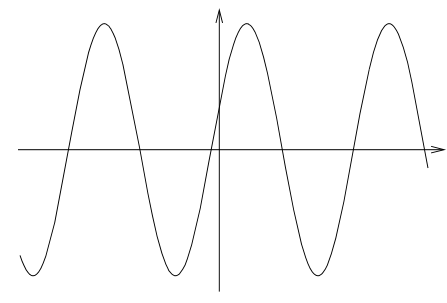
\includegraphics[width=0.6\textwidth]{image//The Genesis of Fourier Analysis//2}
	\caption{The graph of $A \cos (c t-\varphi)$}
	\label{p2}	
\end{figure}
We make two observations regarding our examination of simple harmonic motion. The first is that the mathematical description of the most elementary oscillatory system, namely simple harmonic motion, involves the most basic trigonometric functions $\cos t$ and $\sin t .$ It will be important in what follows to recall the connection between these functions and complex numbers, as given in Euler's identity $e^{i t}=\cos t+i \sin t$. The second observation is that simple harmonic motion is determined as a function of time by two initial conditions, one determining the position, and the other the velocity (specified, for example, at time $t=0$ ). This property is shared by more general oscillatory systems, as we shall see below.

\subsubsection{Standing and traveling waves}
As it turns out, the vibrating string can be viewed in terms of one-dimensional wave motions. Here we want to describe two kinds of motions that lend themselves to simple graphic representations.

- First, we consider standing waves. These are wavelike motions described by the graphs $y=u(x, t)$ developing in time $t$ as shown in $\reffig{p3}$.
\begin{figure}[H]\centering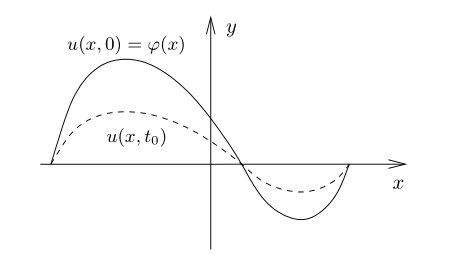
\includegraphics[width=0.6\textwidth]{image//The Genesis of Fourier Analysis//3}
	\caption{A standing wave at different moments in time: $t=0$ and $t=t_{0}$}
	\label{p3}	
\end{figure}

In other words, there is an initial profile $y=\varphi(x)$ representing the wave at time $t=0,$ and an amplifying factor $\psi(t),$ depending on $t$ so that $y=u(x, t)$ with
$$
u(x, t)=\varphi(x) \psi(t)
$$
The nature of standing waves suggests the mathematical idea of "separation of variables," to which we will return later.

- A second type of wave motion that is often observed in nature is that of a traveling wave. Its description is particularly simple:

there is an initial profile $F(x)$ so that $u(x, t)$ equals $F(x)$ when $t=0 .$ As $t$ evolves, this profile is displaced to the right by $c t$ units, where $c$ is a positive constant, namely
$$
u(x, t)=F(x-c t)
$$
Graphically, the situation is depicted in $\reffig{p4}$
\begin{figure}[H]\centering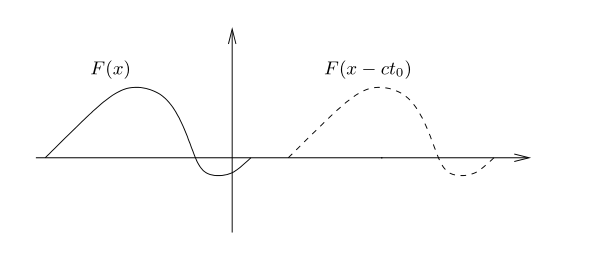
\includegraphics[width=0.6\textwidth]{image//The Genesis of Fourier Analysis//4}
	\caption{A traveling wave at two different moments in time: $t=0$ and $t=t_{0}$}
	\label{p4}	
\end{figure}
Since the movement in $t$ is at the rate $c,$ that constant represents the velocity of the wave. The function $F(x-c t)$ is a one-dimensional traveling wave moving to the right. Similarly, $u(x, t)=F(x+c t)$ is a one-dimensional traveling wave moving to the left.
\subsubsection{Harmonics and superposition of tones}
The final physical observation we want to mention (without going into any details now) is one that musicians have been aware of since time immemorial. It is the existence of harmonics, or overtones. The pure tones are accompanied by combinations of overtones which are primarily responsible for the timbre (or tone color) of the instrument. The idea of combination or superposition of tones is implemented mathematically by the basic concept of linearity, as we shall see below.
\vspace{12pt}

We now turn our attention to our main problem, that of describing the motion of a vibrating string. First, we derive the wave equation, that is, the partial differential equation that governs the motion of the string.

\subsection{ Derivation of the wave equation}
Imagine a homogeneous string placed in the $(x, y)$-plane, and stretched along the $x$-axis between $x=0$ and $x=L .$ If it is set to vibrate, its displacement $y=u(x, t)$ is then a function of $x$ and $t,$ and the goal is to derive the differential equation which governs this function.

For this purpose, we consider the string as being subdivided into a large number $N$ of masses (which we think of as individual particles) distributed uniformly along the $x$-axis, so that the $n^{\text {th }}$ particle has its $x$-coordinate at $x_{n}=n L / N .$ We shall therefore conceive of the vibrating string as a complex system of $N$ particles, each oscillating in the vertical direction only; however, unlike the simple harmonic oscillator we considered previously, each particle will have its oscillation linked to its immediate neighbor by the tension of the string.
\begin{figure}[H]\centering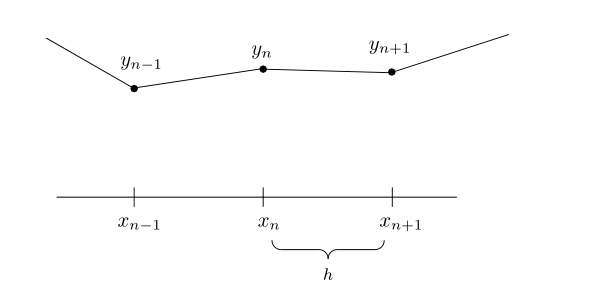
\includegraphics[width=0.6\textwidth]{image//The Genesis of Fourier Analysis//5}
	\caption{A vibrating string as a discrete system of masses}
	\label{p5}	
\end{figure}
We then set $y_{n}(t)=u\left(x_{n}, t\right),$ and note that $x_{n+1}-x_{n}=h,$ with $h=$ $L / N .$ If we assume that the string has constant density $\rho>0,$ it is reasonable to assign mass equal to $\rho h$ to each particle. By Newton's law, $\rho h y_{n}^{\prime \prime}(t)$ equals the force acting on the $n^{\text {th }}$ particle. We now make the simple assumption that this force is due to the effect of the two nearby particles, the ones with $x$-coordinates at $x_{n-1}$ and $x_{n+1}$ (see $\reffig{p5}$). We further assume that the force (or tension) coming from the right of the $n^{\text {th }}$ particle is proportional to $\left(y_{n+1}-y_{n}\right) / h,$ where $h$ is the distance between $x_{n+1}$ and $x_{n}$; hence we can write the tension as
$$
\left(\frac{\tau}{h}\right)\left(y_{n+1}-y_{n}\right)
$$
where $\tau>0$ is a constant equal to the coefficient of tension of the string. There is a similar force coming from the left, and it is
$$
\left(\frac{\tau}{h}\right)\left(y_{n-1}-y_{n}\right)
$$
Altogether, adding these forces gives us the desired relation between the oscillators $y_{n}(t),$ namely
\begin{equation}
\rho h y_{n}^{\prime \prime}(t)=\frac{\tau}{h}\left\{y_{n+1}(t)+y_{n-1}(t)-2 y_{n}(t)\right\}\label{7}
\end{equation}
On the one hand, with the notation chosen above, we see that
$$
y_{n+1}(t)+y_{n-1}(t)-2 y_{n}(t)=u\left(x_{n}+h, t\right)+u\left(x_{n}-h, t\right)-2 u\left(x_{n}, t\right)
$$
On the other hand, for any reasonable function $F(x)$ (that is, one that has continuous second derivatives) we have(泰勒展开)
$$
\frac{F(x+h)+F(x-h)-2 F(x)}{h^{2}} \rightarrow F^{\prime \prime}(x) \quad \text { as } h \rightarrow 0
$$
Thus we may conclude, after dividing by $h$ in $\ref{7}$ and letting $h$ tend to zero (that is, $N$ goes to infinity), that
$$
\rho \frac{\partial^{2} u}{\partial t^{2}}=\tau \frac{\partial^{2} u}{\partial x^{2}}
$$
Or
$$
\frac{1}{c^{2}} \frac{\partial^{2} u}{\partial t^{2}}=\frac{\partial^{2} u}{\partial x^{2}}, \quad \text { with } c=\sqrt{\tau / \rho}
$$
This relation is known as the {\bf one-dimensional wave equation}, or more simply as the wave equation. For reasons that will be apparent later, the coefficient $c>0$ is called the {\bf velocity} of the motion.

In connection with this partial differential equation, we make an important simplifying mathematical remark. This has to do with scaling, or in the language of physics, a "change of units." That is, we can think of the coordinate $x$ as $x=a X$ where $a$ is an appropriate positive constant. Now, in terms of the new coordinate $X,$ the interval $0 \leq x \leq L$ becomes $0 \leq X \leq L / a .$ Similarly, we can replace the time coordinate $t$ by $t=b T$ where $b$ is another positive constant. If we set $U(X, T)=u(x, t),$ then
$$
\frac{\partial U}{\partial X}=a \frac{\partial u}{\partial x}, \quad \frac{\partial^{2} U}{\partial X^{2}}=a^{2} \frac{\partial^{2} u}{\partial x^{2}}
$$
and similarly for the derivatives in $t .$ So if we choose $a$ and $b$ appropriately, we can transform the one-dimensional wave equation into
$$
\frac{\partial^{2} U}{\partial T^{2}}=\frac{\partial^{2} U}{\partial X^{2}}
$$
which has the effect of setting the velocity $c$ equal to $1 .$ Moreover, we have the freedom to transform the interval $0 \leq x \leq L$ to $0 \leq X \leq \pi .$ (We shall see that the choice of $\pi$ is convenient in many circumstances.) All this is accomplished by taking $a=L / \pi$ and $b=L /(c \pi) .$ Once we solve the new equation, we can of course return to the original equation by making the inverse change of variables. Hence, we do not sacrifice generality by thinking of the wave equation as given on the interval $[0, \pi]$ with velocity $c=1.$

\subsection{Solution to the wave equation}
Having derived the equation for the vibrating string, we now explain two methods to solve it:

- using traveling waves,

- using the superposition of standing waves.

While the first approach is very simple and elegant, it does not directly give full insight into the problem; the second method accomplishes that, and moreover is of wide applicability. It was first believed that the second method applied only in the simple cases where the initial position and velocity of the string were themselves given as a superposition of standing waves. However, as a consequence of Fourier's ideas, it became clear that the problem could be worked either way for all initial conditions.

\subsubsection{Traveling waves}
To simplify matters as before, we assume that $c=1$ and $L=\pi,$ so that the equation we wish to solve becomes
$$
\frac{\partial^{2} u}{\partial t^{2}}=\frac{\partial^{2} u}{\partial x^{2}} \quad \text { on } 0 \leq x \leq \pi
$$
The crucial observation is the following: if $F$ is any twice differentiable function, then $u(x, t)=F(x+t)$ and $u(x, t)=F(x-t)$ solve the wave equation.Note that the graph of $u(x, t)=F(x-t)$ at time $t=0$ is simply the graph of $F,$ and that at time $t=1$ it becomes the graph of $F$ translated to the right by
1. Therefore, we recognize that $F(x-t)$ is a traveling wave which travels to the right with speed 1. Similarly, $u(x, t)=F(x+t)$ is a wave traveling to the left with speed $1 .$ These motions are depicted in $\reffig{p6}$.
\begin{figure}[H]\centering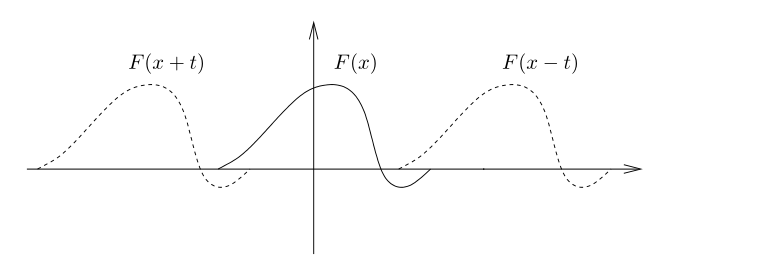
\includegraphics[width=0.6\textwidth]{image//The Genesis of Fourier Analysis//6}
	\caption{Waves traveling in both directions}
	\label{p6}	
\end{figure}

Our discussion of tones and their combinations leads us to observe that the wave equation is {\bf linear}. This means that if $u(x, t)$ and $v(x, t)$ are particular solutions, then so is $\alpha u(x, t)+\beta v(x, t),$ where $\alpha$ and $\beta$ are any constants. Therefore, we may superpose two waves traveling in opposite directions to find that whenever $F$ and $G$ are twice differentiable functions, then
$$
u(x, t)=F(x+t)+G(x-t)
$$
is a solution of the wave equation. In fact, we now show that all solutions take this form.

We drop for the moment the assumption that $0 \leq x \leq \pi,$ and suppose that $u$ is a twice differentiable function which solves the wave equation
for all real $x$ and $t$.(给出真正的通解) Consider the following new set of variables $\xi=x+t$, $\eta=x-t,$ and define $v(\xi, \eta)=u(x, t) .$ The change of variables formula shows that $v$ satisfies
$$
\frac{\partial^{2} v}{\partial \xi \partial \eta}=0
$$
Integrating this relation twice gives $v(\xi, \eta)=F(\xi)+G(\eta),$ which then implies
$$
u(x, t)=F(x+t)+G(x-t)
$$
for some functions $F$ and $G$.
We must now connect this result with our original problem, that is, the physical motion of a string. There, we imposed the restrictions $0 \leq$ $x \leq \pi,$ the initial shape of the string $u(x, 0)=f(x),$ and also the fact that the string has fixed end points, namely $u(0, t)=u(\pi, t)=0$ for all
t. To use the simple observation above, we first extend $f$ to all of $\mathbb{R}$ by making it odd on $[-\pi, \pi],$ and then periodic in $x$ of period $2 \pi,$ and similarly for $u(x, t),$ the solution of our problem. Then the extension $u$ solves the wave equation on all of $\mathbb{R},$ and $u(x, 0)=f(x)$ for all $x \in \mathbb{R}$. Therefore, $u(x, t)=F(x+t)+G(x-t),$ and setting $t=0$ we find that
$$
F(x)+G(x)=f(x)
$$
Since many choices of $F$ and $G$ will satisfy this identity, this suggests imposing another initial condition on $u$ (similar to the two initial conditions in the case of simple harmonic motion), namely the initial velocity of the string which we denote by $g(x)$ :
$$
\frac{\partial u}{\partial t}(x, 0)=g(x)
$$
where of course $g(0)=g(\pi)=0 .$ Again, we extend $g$ to $\mathbb{R}$ first by making it odd over $[-\pi, \pi],$ and then periodic of period $2 \pi .$ The two initial conditions of position and velocity now translate into the following system:
$$
\left\{\begin{array}{l}
F(x)+G(x)=f(x) \\
F^{\prime}(x)-G^{\prime}(x)=g(x)
\end{array}\right.
$$
Differentiating the first equation and adding it to the second, we obtain
$$
2 F^{\prime}(x)=f^{\prime}(x)+g(x)
$$
Similarly
$$
2 G^{\prime}(x)=f^{\prime}(x)-g(x)
$$
and hence there are constants $C_{1}$ and $C_{2}$ so that
$$
F(x)=\frac{1}{2}\left[f(x)+\int_{0}^{x} g(y) d y\right]+C_{1}
$$
and
$$
G(x)=\frac{1}{2}\left[f(x)-\int_{0}^{x} g(y) d y\right]+C_{2}
$$
Since $F(x)+G(x)=f(x)$ we conclude that $C_{1}+C_{2}=0,$ and therefore, our final solution of the wave equation with the given initial conditions takes the form $$
u(x, t)=\frac{1}{2}[f(x+t)+f(x-t)]+\frac{1}{2} \int_{x-t}^{x+t} g(y) d y
$$
The form of this solution is known as {\bf d'Alembert's formula}. Observe that the extensions we chose for $f$ and $g$ guarantee that the string always has fixed ends, that is, $u(0, t)=u(\pi, t)=0$ for all $t$.
(之所以要延拓是为了不再纠结于定义域的问题,从而使最后的代换(f和g的自变量由$x$换成$x+t$或$x-t$)能够严谨顺利地完成,而明确地给出延拓的定义,则是为了保证物理意义:两端的固定点.)

A final remark is in order. The passage from $t \geq 0$ to $t \in \mathbb{R},$ and then back to $t \geq 0$, which was made above, exhibits the time reversal property of the wave equation.(在上面的变化的确没有提到如何从 $t \geq 0$ to $t \in \mathbb{R}$,而最后给出的是$t \geq 0$的情况,则应该要给出$t<0$的定义延拓,这个延拓要保证不会出现新的波动形式) In other words, a solution $u$ to the wave equation for $t \geq 0,$ leads to a solution $u^{-}$ defined for negative time $t<0$ simply by setting $u^{-}(x, t)=u(x,-t),$ a fact which follows from the invariance of the wave equation under the transformation $t \mapsto-t .$ The situation is quite different in the case of the heat equation.


\subsubsection{Superposition of standing waves}
We turn to the second method of solving the wave equation, which is based on two fundamental conclusions from our previous physical observations. By our considerations of standing waves, we are led to look for special solutions to the wave equation which are of the form $\varphi(x) \psi(t)$. This procedure, which works equally well in other contexts (in the case of the heat equation, for instance), is called {\bf separation of variables} and constructs solutions that are called pure tones. Then by the linearity of the wave equation, we can expect to combine these pure tones into a more complex combination of sound. Pushing this idea further, we can hope ultimately to express the general solution of the wave equation in terms of sums of these particular solutions.

Note that one side of the wave equation involves only differentiation in $x,$ while the other, only differentiation in $t .$ This observation provides another reason to look for solutions of the equation in the form $u(x, t)=\varphi(x) \psi(t)$ (that is, to "separate variables"), the hope being to reduce a difficult partial differential equation into a system of simpler ordinary differential equations. In the case of the wave equation, with $u$ of the above form, we get
$$
\varphi(x) \psi^{\prime \prime}(t)=\varphi^{\prime \prime}(x) \psi(t)
$$
and therefore
$$
\frac{\psi^{\prime \prime}(t)}{\psi(t)}=\frac{\varphi^{\prime \prime}(x)}{\varphi(x)}
$$
The key observation here is that the left-hand side depends only on $t$, and the right-hand side only on $x$. This can happen only if both sides are equal to a constant, say $\lambda$. Therefore, the wave equation reduces to the following
\begin{equation}
\left\{\begin{array}{l}
\psi^{\prime \prime}(t)-\lambda \psi(t)=0 \\
\varphi^{\prime \prime}(x)-\lambda \varphi(x)=0
\end{array}\right.\label{8}
\end{equation}
We focus our attention on the first equation in the above system. At this point, we will recognize the equation we obtained in the study of simple harmonic motion. Note that we need to consider only the case when $\lambda<0$, since when $\lambda \geq 0$ the solution $\psi$ will not oscillate as time varies. Therefore, we may write $\lambda=-m^{2},$ and the solution of the equation is then given by
$$
\psi(t)=A \cos m t+B \sin m t
$$
Similarly, we find that the solution of the second equation in $\ref{8}$ is
$$
\varphi(x)=\tilde{A} \cos m x+\tilde{B} \sin m x
$$
Now we take into account that the string is attached at $x=0$ and $x=\pi$. This translates into $\varphi(0)=\varphi(\pi)=0,$ which in turn gives $\tilde{A}=0,$ and if $\tilde{B} \neq 0,$ then $m$ must be an integer. If $m=0,$ the solution vanishes identically, and if $m \leq-1$, we may rename the constants and reduce to the case $m \geq 1$ since the function $\sin y$ is odd and $\cos y$ is even. Finally, we arrive at the guess that for each $m \geq 1,$ the function
$$
u_{m}(x, t)=\left(A_{m} \cos m t+B_{m} \sin m t\right) \sin m x
$$
which we recognize as a standing wave, is a solution to the wave equation. Note that in the above argument we divided by $\varphi$ and $\psi$, which sometimes vanish, so one must actually check by hand that the standing wave $u_{m}$ solves the equation.

Before proceeding further with the analysis of the wave equation, we pause to discuss standing waves in more detail. The terminology comes from looking at the graph of $u_{m}(x, t)$ for each fixed $t .$ Suppose first that $m=1,$ and take $u(x, t)=\cos t \sin x .$ Then, $\reffig{p7}(a)$ gives the graph of $u$ for different values of $t$.
\begin{figure}[H]\centering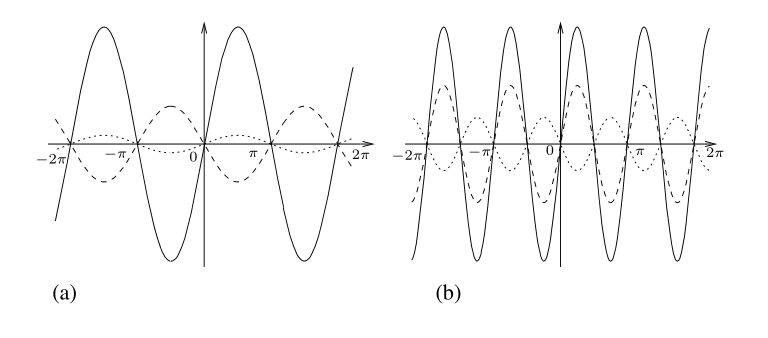
\includegraphics[width=1\textwidth]{image//The Genesis of Fourier Analysis//7}
	\caption{Fundamental tone (a) and overtones (b) at different moments in time}
	\label{p7}	
\end{figure}
The case $m=1$ corresponds to the {\bf fundamental tone} or {\bf first harmonic} of the vibrating string.

We now take $m=2$ and look at $u(x, t)=\cos 2 t \sin 2 x .$ This corresponds to {\bf the first overtone} or {\bf second harmonic}, and this motion is described in $\reffig{p7}(b)$. Note that $u(\pi / 2, t)=0$ for all $t$. Such points, which remain motionless in time, are called nodes, while points whose motion has maximum amplitude are named anti-nodes.

For higher values of $m$ we get more overtones or higher harmonics. Note that as $m$ increases, the frequency increases, and the period $2 \pi / m$ decreases. Therefore, the fundamental tone has a lower frequency than the overtones.

We now return to the original problem. Recall that the wave equation is linear in the sense that if $u$ and $v$ solve the equation, so does $\alpha u+\beta v$ for any constants $\alpha$ and $\beta$. This allows us to construct more solutions by taking linear combinations of the standing waves $u_{m} .$ This technique, called superposition, leads to our final guess for a solution of the wave equation
\begin{equation}
u(x, t)=\sum_{m=1}^{\infty}\left(A_{m} \cos m t+B_{m} \sin m t\right) \sin m x
\end{equation}
Note that the above sum is infinite, so that questions of convergence arise, but since most of our arguments so far are formal, we will not worry about this point now.

Suppose the above expression gave all the solutions to the wave equation. If we then require that the initial position of the string at time $t=0$ is given by the shape of the graph of the function $f$ on $[0, \pi],$ with of course $f(0)=f(\pi)=0,$ we would have $u(x, 0)=f(x),$ hence
$$
\sum_{m=1}^{\infty} A_{m} \sin m x=f(x).$$
Since the initial shape of the string can be any reasonable function $f,$ we must ask the following basic question:
Given a function $f$ on $[0, \pi]$ (with $f(0)=f(\pi)=0$ ), can we find coefficients $A_{m}$ so that
\begin{equation}
f(x)=\sum_{m=1}^{\infty} A_{m} \sin m x ?\label{9}
\end{equation}
This question is stated loosely, but a lot of our effort will be to formulate the question precisely and attempt to answer it. This was the basic problem that initiated the study of Fourier analysis.

A simple observation allows us to guess a formula giving $A_{m}$ if the expansion $\ref{9}$ were to hold. Indeed, we multiply both sides by $\sin n x$ and integrate between $[0, \pi]$; working formally, we obtain
$$
\begin{aligned}
\int_{0}^{\pi} f(x) \sin n x d x &=\int_{0}^{\pi}\left(\sum_{m=1}^{\infty} A_{m} \sin m x\right) \sin n x d x \\
&=\sum_{m=1}^{\infty} A_{m} \int_{0}^{\pi} \sin m x \sin n x d x=A_{n} \cdot \frac{\pi}{2}
\end{aligned}
$$
where we have used the fact that
$$
\int_{0}^{\pi} \sin m x \sin n x d x=\left\{\begin{array}{ll}
0 & \text { if } m \neq n \\
\pi / 2 & \text { if } m=n
\end{array}\right.
$$
(用$\cos(m+n)$和$\cos(m-n)$改写式子)

Therefore, the guess for $A_{n},$ called the $n^{\text {th }}$ Fourier sine coefficient of $f$, is
\begin{equation}
A_{n}=\frac{2}{\pi} \int_{0}^{\pi} f(x) \sin n x d x
\end{equation}
We shall return to this formula. and other similar ones, later.

























\end{document}
